\documentclass[12pt,a4paper,twoside]{book}
\usepackage{amsmath}
\usepackage{setspace}
\usepackage{geometry}
\usepackage{times}
\usepackage{fancyhdr}
\usepackage[utf8x]{inputenc}
\usepackage{graphicx}
\usepackage{xcolor}
\usepackage{listings}
\usepackage{makecell}
\usepackage{xcolor,colortbl}
\usepackage{caption}
\captionsetup[table]{position=bottom} 
\graphicspath{ {immagini/} }
\fancyhf{} % clear all header and footers
\renewcommand{\headrulewidth}{0pt} % remove the header rule
\fancyfoot[LE,RO]{\thepage} % Left side on Even pages; Right side on Odd pages
\pagestyle{fancy}
\fancypagestyle{plain}{%
  \fancyhf{}%
  \renewcommand{\headrulewidth}{0pt}%
  \fancyhf[lef,rof]{\thepage}%
}

\usepackage{pdfpages}
\usepackage[italian]{babel}
\usepackage[hyphens,spaces,obeyspaces]{url}
\usepackage[hidelinks]{hyperref}
\usepackage[T1]{fontenc}

\usepackage{float}

\usepackage{titlesec}
\titleformat{\chapter}[hang] 
{\normalfont\huge\bfseries}{\chaptertitlename\ \thechapter:}{1em}{} 
\renewcommand{\chaptername}{Capitolo}

\colorlet{punct}{red!60!black}
\definecolor{background}{HTML}{EEEEEE}
\definecolor{delim}{RGB}{20,105,176}
\colorlet{numb}{magenta!60!black}
\lstdefinelanguage{json}{
	basicstyle=\normalfont\ttfamily,
	numbers=left,
	numberstyle=\scriptsize,
	stepnumber=1,
	numbersep=8pt,
	showstringspaces=false,
	breaklines=true,
	frame=lines,
	backgroundcolor=\color{background},
	literate=
	*{0}{{{\color{numb}0}}}{1}
	{1}{{{\color{numb}1}}}{1}
	{2}{{{\color{numb}2}}}{1}
	{3}{{{\color{numb}3}}}{1}
	{4}{{{\color{numb}4}}}{1}
	{5}{{{\color{numb}5}}}{1}
	{6}{{{\color{numb}6}}}{1}
	{7}{{{\color{numb}7}}}{1}
	{8}{{{\color{numb}8}}}{1}
	{9}{{{\color{numb}9}}}{1}
	{:}{{{\color{punct}{:}}}}{1}
	{,}{{{\color{punct}{,}}}}{1}
	{\{}{{{\color{delim}{\{}}}}{1}
	{\}}{{{\color{delim}{\}}}}}{1}
	{[}{{{\color{delim}{[}}}}{1}
	{]}{{{\color{delim}{]}}}}{1},
	otherkeywords = {uid,@context,@type,permission,target, action, prohibition, assigner, assignee, profile,@id,dc,title,odrl,partOf,vcard,fn,hasEmail,rdf,value,refinement,leftOperand,
	operator,rightOperand,unit,xone,@list,resource,source,constraint,Permission,
	rdfs,Class,isDefinedBy,label,subClassOf,about,type,Prohibition},
    keywordstyle = {\textbf},
}
\definecolor{pblue}{rgb}{0.13,0.13,1}
\definecolor{pgreen}{rgb}{0,0.5,0}
\definecolor{pred}{rgb}{0.9,0,0}
\definecolor{pgrey}{rgb}{0.46,0.45,0.48}
\lstset{language=Java,
  frame=single, 
  numbers=left,
	numberstyle=\scriptsize,
	stepnumber=1,
	numbersep=8pt,
  showspaces=false,
  showtabs=false,
  breaklines=true,
  showstringspaces=false,
  breakatwhitespace=true,
  commentstyle=\color{pgreen},
  keywordstyle=\color{pblue},
  stringstyle=\color{pred},
  basicstyle=\ttfamily,
  moredelim=[il][\textcolor{pgrey}]{$$},
  moredelim=[is][\textcolor{pgrey}]{\%\%}{\%\%}
}




\geometry{a4paper,top=3cm,bottom=3cm,left=3cm,right=3cm,heightrounded,bindingoffset=5mm}
\onehalfspacing
\title{Aggiunta della semantica per merging di policy in ODRL }
\date{28 giugno 2020}
\author{Gianluca Oldani}

\begin{document}
\maketitle
\tableofcontents
\chapter{Introduzione}
Questo lavoro di tesi si inserisce all'interno del contesto del progetto europeo \textit{Multi-Owner data Sharing for Analytics and Integration respecting Confidentiality and OWNer control} (MOSAICrOWN). Come da titolo, il progetto nasce come risposta all'esigenza di ricercare metodi per la realizzazione di mercati digitali relativi allo scambio di dati, garantendo il rispetto delle norme vigenti in materia di privacy ed eventuali requisiti di riservatezza espressi dagli utenti finali in un ambiente multi-owner. Questa tesi si inserisce all'interno del pacchetto di lavoro \textit{Policy specifications - Data governance framework}, il quale si occupa della definizione di un linguaggio, e relativo modello, per la definizione di requisiti di privacy; questo componente risulta critico poiché interessa l'intero ciclo di vita del dato, oltre ad influenzare l'operato degli altri due \textit{work package}. Tra i candidati esaminati per la definizione di questi metadati vi è l' \textit{Open Digital Rights Language} (ODRL). Inizialmente, il lavoro di tesi si occupa di esaminare la struttura del linguaggio ed evidenziarne due problematiche all'interno del contesto di MOSAICrOWN. La prima problematica risulta essere l'assenza di una gestione dei conflitti efficace in scenari multi-owner; la seconda problematica risulta essere l'inefficiente rappresentazione delle regole in fase di interrogazione del modello.\\
Individuate queste problematiche, la tesi mostra quali sono le tecnologie ed i principi che hanno guidato l'implementazione di una soluzione. La proposta consiste in un tool che attua il \textit{merging} di due policy qualora queste operino sulla stessa risorsa; prima di procedere all'effettiva implementazione, sono state individuate le varie casistiche possibili ed esempi degli scenari in cui si presentano, al fine di caratterizzare al meglio la problematica.\\Dopo questa caratterizzazione, il lavoro di tesi espone l'architettura della soluzione implementata, mostrando schemi UML e pseudocodice Java-like per dimostrare l'efficacia e la modularità della proposta nelle parti più importanti.\\
L'ultimo capitolo della tesi si concentra sulla valutazione dei risultati ottenuti, riassumendo quali fossero le problematiche affrontate e mostrando i vantaggi del tool creato tramite un confronto con una soluzione baseline in una serie di scenari dalla complessità crescente.
\chapter{Il progetto MOSAICrOWN}
Il progetto MOSAICrOWN nasce come risposta all'esigenza di ricercare metodi per la realizzazione di mercati digitali relativi allo scambio di dati\cite{ProgettoMosaico}. In particolare, si inserisce nel contesto relativo alle sfide introdotte dai requisiti di privacy che è necessario garantire in queste applicazioni. Questi requisiti rappresentano ostacoli per task quali: aggregazione di dati posseduti da più attori, analisi di dati.\\
Gli obiettivi che il progetto si pone sono:
\begin{itemize}
\item peremttere lo scambio di dati in sicurezza, sia per quanto concerne la protezione di informazioni personali che informazioni sensibili in ambito aziendale;
\item dare supporto a realtà in cui vi è carenza di skills in ambito gestione dati, fornendo la possibilità ai possessori delle risorse di usufruire di strumenti per la protezione, scambio ed analisi dei dati;
\item standardizzare le procedure di scambio di dati tra diverse realtà in ambito europeo.
\end{itemize}
Il metodo con cui si intende realizzare questi obiettivi risulta essere la creazione di un framework che permetta la definizione di requisiti relativi alla protezione dei dati in modo dichiarativo; tali requisiti sono poi utilizzati durante l'intero ciclo di vita del dato per mettere in atto tecniche di protezione. Le procedure utilizzate devono, inoltre, risultare efficienti, scalabili ed essere realizzate con in mente uno scenario che pone l'attenzione sulla privacy in ambienti multi-owner.\\
Altri aspetti che il progetto MOSAICrOWN tiene in considerazione sono:
\begin{itemize}
\item implementazione adatta al deployment in sistemi reali, cercando di adottare le migliore tecniche che la ricerca ha da offrire nella tutela della privacy;
\item indipendenza del framework dalla specifica piattaforma in cui viene impiegato, cercado di supportare come casi d'uso principali:
\begin{itemize}
\item una sola entità che gestisce il mercato digitale e che offre strumenti di analisi dei dati;
\item una sola entità che gestisce il mercato digitale ma che demanda l'analisi dei dati ad entità esterne.
\end{itemize}
\item varietà dei gradi di sicurezza garantiti in relazione al degrado di performance introdotto dalle tecniche di protezione impiegate, permettendo così agli utilizzatori di gestire un trade-off tra certificazioni sulla privacy e valore dei dati.
\end{itemize}

\section{Architettura del progetto}
Il progetto modella il ciclo di vita del dato individuandone tre fasi:
\begin{enumerate}
\item \textbf{ingestion}: il dato passa dal suo possessore al mercato digitale; in questa fase si punta a fornire tecnologie che permettano al data owner di specificare le restrizioni che devono essere rispettate sui dati inseriti nel mercato e, inoltre, si dà la possibilità di attuare tecniche che diano garanzie sul rispetto di questi requisiti; queste ultime tecnologie supportano scenari dove l'entità che possiede il mercato digitale non è un soggetto trusted.
\item \textbf{storage}: il dato è conservato e gestito dall'entità che comanda il mercato digitale; le tecnologie fornite in questa fase puntano a proteggere il dato sia durante la conservazione, sia durante l'interrogazione del dato; in questa fase risulta importante garantire l'interoperabilità con altri ambienti che non fanno uso di questi strumenti. Particolare attenzione viene data all'evitare il degrado delle performance quando si opera su dati protetti con granularità fine.
\item \textbf{analytics}: il dato è processatto all'interno del mercato digitale; in questa fase le tecnologie fornite permettono ai vari possessori di effettuare analisi sui dati in maniera efficiente, basandosi sull'entità richiedente e sui requisiti di protezione specificati per i dati.
\end{enumerate}
A livello implementativo il progetto è diviso in tre \textit{work package}:
\begin{enumerate}
\label{tesiWP}
\item \textbf{Policy specifications - Data governance framework}: questo pacchetto di lavoro si pone come obiettivo la definizione di un framework per la gestione e la specifica di policy in scenari di aggregazione dati multi-owner. Il fine è rendere possibile ai possessori dei dati la regolazione dell'uso che è possibile fare sui propri asset sviluppando un linguaggio, ed un relativo modello, per la dichiarazione di policy. Sia il modello che il linguaggio devono risultare flessibili, poiché i requisiti espressi devono riguardare ogni fase della vita del dato.
\item \textbf{Data wrapping}: questo pacchetto di lavoro si preoccupa della definizione di tecniche che permettano l'accesso ai dati in modo efficiente ma che non compromettano i requisiti di protezione specificati mediante il modello fornito nel package precedente. Particolare enfasi è data sull'evitare la re-identificazione dei dati;
\item \textbf{Data sanitisation}: quest'ultimo pacchetto di lavoro mira alla definizione di tecniche efficienti e scalabili che operino su intere collezioni di dati, al fine di offrirne una versione offuscata e/o aggregata che sia robusta ad attacchi che mirano a compremetterne la privacy e/o la confidenzialità. Questo package mira anche a fornire tecniche che permettano di valutare il grado di protezione di un dato in relazione al valore che questo mantiene. 
\end{enumerate}
Tutti i tre workpackage esposti devono essere impiegabili in ogni fase del ciclo di vita del dato, come mostrato nella seguente figura:
\begin{figure}[H]
\centering
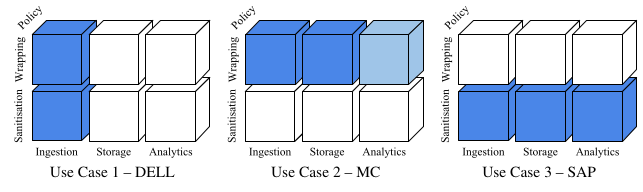
\includegraphics[scale=.65]{../immagini/MOSAICOUSES.png}
\caption{Caratterizzazione dei casi d'uso presi in considerazione da MOSAICrOWN\cite{ProgettoMosaico}}
\label{MosUses}
\end{figure}
\section{Scenari d'uso}
Lo sviluppo del progetto si basa sul soddisfare i requisiti di tre scenari individuati; ogni caso studio prende in considerazione uno specifico tipo di attore che può prendere parte ad un mercato digitale. Come visibile anche all'interno della figura \ref{MosUses}, gli scenari affrontati sono:
\begin{itemize}
\item \textbf{DELL}: in questo caso d'uso si affronta la problematica dal punto di vista dei possessori di dati; per questi attori risulta cruciale la possibilità di definire requisiti di privacy e legislativi sui propri dati e poter sfruttare tecniche che assicurino questi requisiti anche in ambienti non trusted. Questi utenti sono interessati solamente dalla fase di \textit{ingestion} ma sfruttano ogni tecnologia all'interno del progetto;
\item \textbf{MasterCard}: in questo caso d'uso si affronta la problematica dal punto di vista di un gestore di una piattaforma per l'analisi dei dati; per questi attori è cruciale il rispetto delle norme vigenti in termini di privacy ed, allo stesso tempo, poter fornire dati di qualità anche con granularità fine; questo tipo di utenti ha il controllo sull'intero ciclo di vita di un dato, con la possibilità di far effettuare l'analisi dei dati ad altre entità; data la granularità del dato, non è necessario l'uso del layer di \textit{data sanitisation};
\item \textbf{SAP}: in questo caso d'uso si affronta la problematica dal punto di vista di un gestore di una piattaforma per lo storage dei dati; per questi attori è cruciale il rispetto delle norme vigenti in termini di privacy e poterne misurare l'efficacia; questo tipo di utenti ha il controllo sull'intero ciclo di vita di un dato; data la granularità del dato, non è necessario l'uso del layer di \textit{data wrapping}.
\end{itemize}
\section{Collocamento del lavoro di tesi}
Questa tesi si colloca all'interno degli studi effettuati per l'implementazione del pacchetto di lavoro denominato \textit{Policy specifications - Data governance framework}. In particolare viene analizzato uno dei linguaggi candidati per la modellizzazione dei requisiti di privacy: l' Open Digital Rights Language (ODRL), le cui proprietà sono trattate nel capitolo \ref{ODRLChapter}.\\
Le motivazioni per cui questo linguaggio risulta un candidato interessante sono:
\begin{itemize}
\item l'essere uno standard definito dal W3C, patner del progetto ed importante risorsa per la standardizzazione delle soluzioni prodotte da MOSAICrOWN;
\item la possibilità di implementazione mediante l'uso di linguaggi di definizione di metadati diffusi, quali XML ed JSON;
\item l'essere nato come linguaggio per l'espressioni di policy, senza assunzioni di contesti specifici;
\item l'essere utilizzato all'interno dell'industria del settore \textit{Digital rights management} (DRM).
\end{itemize}
Questo \textit{work package} è fondamentale in ogni fase di vita del dato ed, inoltre, è necessario in tutti i casi d'uso individuati; alla luce di ciò, la comprensione dei punti di forza e delle limitazioni del modello risultano aspetti cruciali per il progetto MOSAICrOWN. \\
ODRL soddisfa sia il requisito di flessibilità che di vicinanza alle tecnologie attualmente in essere.
\chapter{ODRL}\label{ODRLChapter} 
\section{Il linguaggio}
\subsection{Definizione ed obiettivi}
``L' Open Digital Rights Language (ODRL) è un linguaggio per l'espressione di policy che definisce: un modello dell'informazione flessibile ed interoperativo, un vocabolario e un meccanismo di codifica per la rappresentazione delle istruzioni sull'uso di contenuti o servizi''\cite{ODRLinfMod}.\\
Il linguaggio si pone all'interno dello scenario applicativo nel quale vi è la necessità di definire:
\begin{itemize}
	\item quali azioni siano permesse o proibite su una risorsa. Queste regole possono essere imposte da leggi o direttamente dal possessore dell'asset o servizio;
	\item indicare quali attori interagiscono con le policy definite; in particolare chi può definire le policy e a chi si applicano le regole al suo interno;
	\item indicare eventuali vincoli riguardanti i permessi ed i divieti espressi.
\end{itemize}
Avere un modello standard per definire questi bisogni dà due vantaggi:
\begin{itemize}
	\item chi possiede l'asset è in grado di definire in modo chiaro quali siano le azioni che un consumatore può fare, evitandone utilizzi indesiderati;
	\item chi usufruisce dell'asset conosce in modo preciso quali azioni può compiere, evitando così di infrangere regole o leggi.
\end{itemize}
ODRL definisce un modello semantico di permessi, divieti ed obblighi che può essere usato per descrivere le modalità d'uso di un contenuto. In particolare cerca di definire i concetti chiave per la creazione di policy machine-readable collegate direttamente all'asset al quale sono associate: ciò permette all'utente finale di reperire facilmente informazioni sulla risorsa alla quale si accede. Quest'ultima proprietà è fondamentale per comprendere il linguaggio, poiché ODRL è costruito seguendo i \textit{Linked Data principles}\cite{LinkedDataInfo}:
\begin{itemize}\label{linkedDataPrinc}
\item utilizzo di URIs come identificativi per le risorse;
\item gli URI sono indirizzi HTTP, così che si possano cercare informazioni sulle risorse;
\item l'URI deve fornire informazioni utili sulla risorsa;
\item tra le informazioni si cerca di fornire altri URI, in modo che l'utente possa raggiungere altre risorse.
\end{itemize}
Nonostante questi principi siano più indicati per un'implementazione graph-based, è possibile anche definire utilizzi che non tengano conto dei link tra le varie informazioni inserite nel documento ODRL.
\subsection{Il modello}\label{modello}
\begin{figure}[H]
	\centering
	\def\svgwidth{\columnwidth}
	\scalebox{0.5}{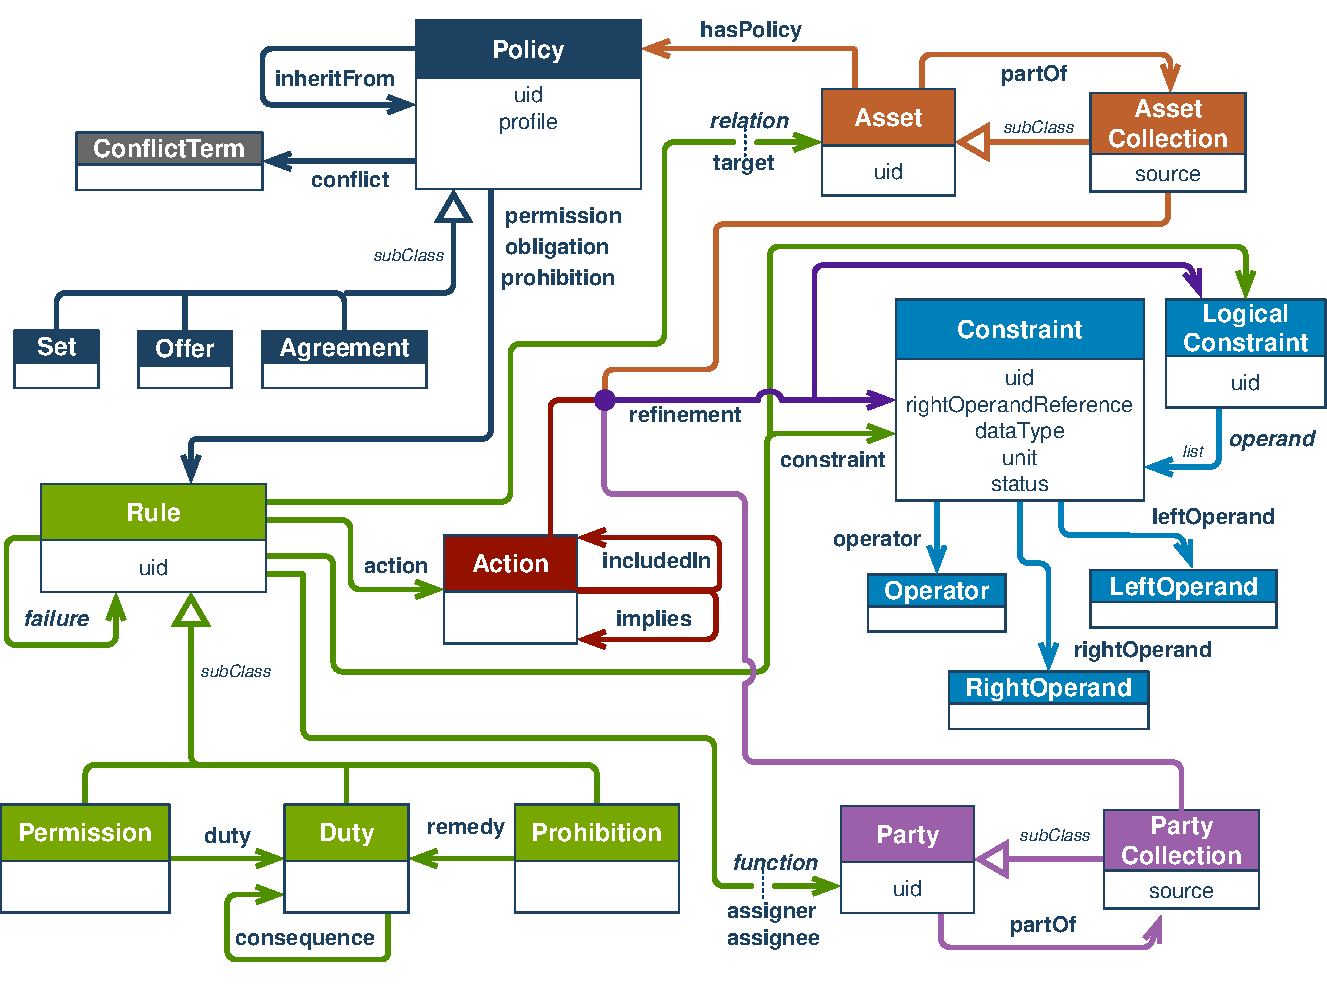
\includegraphics{ODRLModel}}
	
	\caption{Schema del modello ODRL\cite{ODRLinfMod}\label{ODRLModelSchema}}
\end{figure}
Come visibile all'interno dello schema in figura \ref{ODRLModelSchema}, il modello è basato sulle seguenti entità principali:
\begin{itemize}
	\item \textbf{Policy}: un gruppo di una o più regole;
	\item \textbf{Regola}: concetto astratto che racchiude le caratteristiche comuni di \textbf{permesso}, \textbf{divieto} e \textbf{dovere};
	\item \textbf{Asset}: risorsa o collezione di risorse soggette a regole;
	\item \textbf{Azione}: operazione su un asset;
	\item \textbf{Party}: entità o insieme di entità con un certo ruolo in una regola;
	\item \textbf{Vincoli}: espressione logica o booleana imposta su azioni, party, asset o regole.
\end{itemize}
\paragraph{Vocabolari}\mbox{}\\
\label{profili}
``L' \textit{ODRL Vocabulary and Expression} descrive i termini usati dalle policy ODRL e come codificarle''\cite{ODRVocab}. All'interno di ODRL, i vocabolari utilizzati per definire i termini all'interno delle policy vengono detti \textbf{profili}, i quali possono essere usati per definire termini che supportano specifiche applicazioni; all'interno di un profilo è possibile, ad esempio, fornire le specifiche riguardanti nuove sottoclassi di termini già presenti nei vocabolari standard di ODRL. I due vocabolari principali definiti sono:
\begin{itemize}
	\item \textbf{ODRL Core Vocabulary}: rappresenta l'insieme minimo di termini per l'espressione di policy supportato;
	\item \textbf{ODRL Common Vocabulary}: arricchisce il vocabolario precedente con gruppi di \textit{azioni}, \textit{sottoclassi} per le policy, \textit{ruoli} per i party e \textit{relazioni} tra gli asset.
\end{itemize}
Una delle principali differenze tra i due vocabolari la si ha all'interno delle \textbf{azioni} che possono essere indicate: nel primo caso si hanno a disposizione solamente due azioni \textbf{use} e \textbf{transfer}, nel secondo caso queste azioni vengono estese da altre azioni figlie, come mostrato in figura \ref{imgUseTransfer}.

\begin{figure}[H]
	\centering
	\def\svgwidth{\columnwidth}
	\scalebox{0.35}{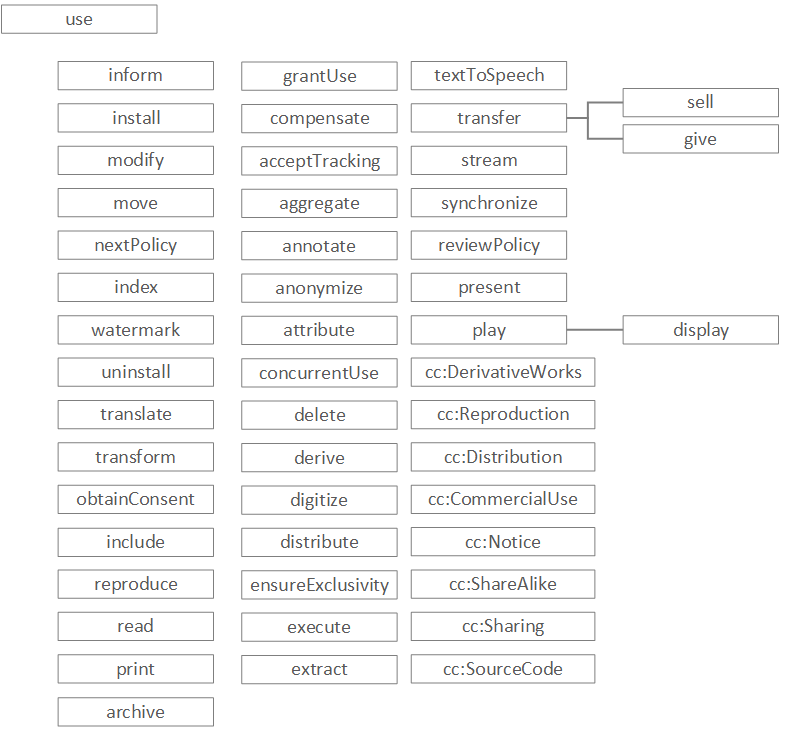
\includegraphics{useTree}}
	
	\caption{Tutte le azioni mostrate sono figlie di \textbf{use}, ad eccezione di \textbf{trasfer} e le sue sottoazioni\cite{ODRLBestPract}\label{imgUseTransfer}}
\end{figure}


\paragraph{Policy}\mbox{}\\
Come definito nel modello presente nella sezione \ref{modello}, una policy è un gruppo non vuoto di \textbf{regole} e, quindi, di \textbf{permessi}, \textbf{divieti} o \textbf{obblighi}. Una policy deve soddisfare i seguenti requisiti:
\begin{itemize}
	\item deve avere un identificativo univoco, inserito nel campo \textbf{uid};
	\item deve avere almeno una regola;
	\item può specificare un profilo; campo obbligatorio se non si usa il Core Vocabulary descritto nella sezione \ref{profili};
	\item può specificare una policy da cui eredita le proprietà;
	\item può specificare una strategia per la risoluzione dei conflitti.
\end{itemize}
Come visibile dalla figura \ref{ODRLModelSchema}, una policy ha tre prossibili sottoclassi:
\begin{itemize}
	\item \textbf{Set}: un insieme di regole che hanno effetto;
	\item \textbf{Agreement}: regole concesse ad una entità assegnataria da una assegnatrice;
	\item \textbf{Offer}: proposta di una regola da parte di un assegnatore.
\end{itemize}
Di seguito un esempio di policy definita mediante ODRL:
\begin{lstlisting}[language=json,firstnumber=1,caption={Policy con sottoclasse \textbf{Set}},captionpos=b,label=esmpioPolicy]
{
 "@context": "http://www.w3.org/ns/odrl.jsonld",
 "@type": "Set",
 "uid": "http://example.com/policy:1010",
 "permission": [{
   "target": "http://example.com/asset:9898.movie",
   "action": "use"
 }]
}
\end{lstlisting}
Dalla policy mostrata nel listing \ref{esmpioPolicy} si può notare:
\begin{itemize}
	\item @type: serve ad indicarne la sottoclasse;
	\item non usando termini fuori dai due vocabolari principali, non necessita la definizione di un profilo;
	\item l'id univoco è rappresentato da un URL che conduce ad informazioni relative alla risorsa.
\end{itemize}
\paragraph{Asset}\mbox{}\\
Come definito nel modello presente nella sezione \ref{modello}, un asset è una risorsa o una collezione di risorse soggette a regole. Un asset può essere una qualsiasi entità identificabile. Ha \textbf{AssetCollection} come sottoclasse, la quale rappresenta una collezione di asset. La classe asset può avere:
\begin{itemize}
\item un identificativo univoco, il quale può essere omesso se l'asset è fornito direttamente con la policy; le specifiche di ODRL, pur supportando questo caso d'uso, sconsigliano questa pratica;
\item una o più proprietà denominate \textbf{partOf}: identifica le collezioni di cui fa parte l'asset, il quale può essere a sua volta una collezione.
\end{itemize}
Esempio di utilizzo in una regola:
\begin{lstlisting}[language=json,firstnumber=1,caption={Utilizzo di asset nella proprietà \textbf{target} di una regola},captionpos=b,label=esempioAsset]
{
"@context": "http://www.w3.org/ns/odrl.jsonld",
 "@type": "Offer",
 "uid": "http://example.com/policy:3333",
 "profile": "http://example.com/odrl:profile:02",
 "permission": [{
	"target": "http://example.com/archive:1011",
	"action": "display",
	"assigner": "http://example.com/party:0001"
 }]
}
\end{lstlisting}
La sottoclasse \textbf{AssetCollection} può avere i seguenti campi aggiuntivi:
\begin{itemize}
	\item \textbf{source}: sostituisce il campo \textbf{uid} nelle classe \textit{AssetCollection} all'interno di un \textbf{refinement};
	\item uno o più \textbf{refinement}: vincoli riguardanti la collezione che identificano solamente un sottogruppo di asset al suo interno.
\end{itemize}
\newpage
Esempio di utilizzo della proprietà \textbf{partOf}:
\begin{lstlisting}[language=json,firstnumber=1,caption={L'asset definito è parte del target presente nel listing \ref{esempioAsset}},captionpos=b,label=esempioAssetColl]
{
	"@type": "dc:Document",
	"@id": "http://example.com/asset:111.doc",
	"dc:title": "Annual Report",
	...
	"odrl:partOf": "http://example.com/archive:1011",
	...
}
\end{lstlisting}
In quest'ultimo esempio si ha che l'asset con id \\``\url{http://example.com/asset:111.doc}''\\è definito come parte della collezione\\``\url{http://example.com/archive1011}''\\Questa definizione ha come effetto l'applicarsi della policy presente nel listing \ref{esempioAsset} anche all'asset figlio.
\paragraph{Party}\mbox{}\\
Come definito nel modello presente nella sezione \ref{modello}, un party è una entità o una collezione di entità con funzione di assegnatario o assegnatore in una regola. Un party può essere un qualunque soggetto con un ruolo attivo nelle regole o che produce un effetto specifico; ad esempio può essere chi controlla che le azione relative ad un dovere vengano rispettate. Presenta \textbf{PartyCollection} come sottoclasse, la quale rappresenta una collezione di entità. La classe party può avere:
\begin{itemize}
	\item un identificativo univoco, il quale può essere omesso se è possibile definire in altro modo l'entità; le specifiche di ODRL, pur supportando questo caso d'uso, sconsigliano questa pratica;
	\item una o più proprietà denominate \textbf{partOf}: identifica le collezioni di cui fa parte l'entità, la quale può essere a sua volta una collezione.
\end{itemize}\newpage
Esempio di utilizzo in una regola:
\begin{lstlisting}[language=json,firstnumber=1,caption={Utilizzo di party nelle proprietà \textbf{assigner} ed \textbf{assignee} di una regola},captionpos=b,label=esempioParty]
{
"@context": "http://www.w3.org/ns/odrl.jsonld",
"@type": "Agreement",
"uid": "http://example.com/policy:8888",
"profile": "http://example.com/odrl:profile:04",
"permission": [{
"target": "http://example.com/music/1999.mp3",
"assigner": "http://example.com/org/sony-music",
"assignee": "http://example.com/people/billie",
"action": "play"
}]
}  
\end{lstlisting}
La sottoclasse \textbf{PartyCollection} può avere i seguenti campi aggiuntivi:
\begin{itemize}
	\item \textbf{source}: sostituisce il campo \textbf{uid} nelle classe PartyCollection all'interno di un \textbf{refinement};
	\item uno o più \textbf{refinement}: vincoli riguardanti la collezione che identificano solamente un sottogruppo di entità al suo interno.
\end{itemize}
Esempio di utilizzo della proprietà \textbf{partOf}:
\begin{lstlisting}[language=json,firstnumber=1,caption={L'entità definita è parte di una PartyCollection},captionpos=b,label=esempioPartyColl]
{
"@type": "vcard:Individual",
"@id": "http://example.com/person/murphy",
"vcard:fn": "Murphy",
"vcard:hasEmail": "murphy@example.com",
...
"odrl:partOf": "http://example.com/team/A",
...
}
\end{lstlisting}
In quest'ultimo esempio si ha che l'entità con id \\``\url{http://example.com/person/murphy}''\\è definita come parte della collezione\\``\url{http://example.com/team/A}''. Questa definizione ha come effetto l'affidare le funzioni di quest'ultima anche alla singola entità.
\paragraph{Action}\mbox{}\\
Come definito nel modello presente nella sezione \ref{modello}, \textbf{action} è una classe che rappresenta un'operazione che può essere esercitata su un asset, al quale viene associata mediante la propietà \textbf{action} di una regola. Nell' ODRL Core Vocabulary sono presenti due azioni principali:
\begin{itemize}
	\item use: un qualsiasi utilizzo dell'asset;
	\item transfer: una qualsiasi azione che preveda il trasferimento di proprietà dell'asset;
\end{itemize}
Un'azione può avere le seguenti proprietà:
\begin{itemize}\label{includesProp}
	\item refinement: raffinamenti semantici sull'azione, come ad esempio l'ammontare di un pagamento, il luogo nel quale l'azione può essere eseguita o il tempo massimo di esecuzione;
	\item includedIn: esprime l'azione padre; la conseguenza di questa dichiarazione risulta essere che tutte le regole applicate all'azione padre, devono valere anche per l'azione figlia;
	\item implies: esprime un'azione che non deve essere vietata per permettere l'azione con questa proprietà; le due azioni non hanno una relazione espressa tramite \textit{includedIn}\footnote{attualmente né l'ODRL Core Vocabulary né l'ODRL Common Vocabulary presentano azioni con questa proprietà}. 
\end{itemize}
Come anticipato nel paragrafo \ref{profili} relativo ai profili, l'ORDL Common Vocabulary utilizza la proprietà \textit{includedIn} per aggiungere azioni figlie sia ad \textit{use} che \textit{transfer}, come già mostrato nella figura \ref{imgUseTransfer}.\\
Di seguito un esempio di azione in una regola:
\begin{lstlisting}[language=json,firstnumber=1,caption={L'azione \textbf{play} è presente nella proprietà \textbf{action} della regola},captionpos=b,label=esempioAction]
{
 "@context": "http://www.w3.org/ns/odrl.jsonld",
 "@type": "Offer",
 "uid": "http://example.com/policy:1012",
 "profile": "http://example.com/odrl:profile:06",
 "permission": [{
  "target": "http://example.com/music:1012",
  "assigner": "http://example.com/org:abc",
  "action": "play"
 }]}
\end{lstlisting}
\label{ConstraintODRL}
\paragraph{Constraint e Logical Constraint}\mbox{}\\
Come definito nel modello presente nella sezione \ref{modello}, \textbf{constraint} è una classe usata per comparare due espressioni che non sono constraint a loro volta, utilizzando un operatore relazionale. Rappresentano una limitazione tramite un confronto, la quale può essere soddisfatta o non soddisfatta. La classe presenta le seguenti proprietà:
\begin{itemize}
	\item uno o nessun identificativo univoco, qualora si volesse riutilizzare l'espressione di confronto definita;
	\item un \textbf{leftOperand}: elemento a sinistra dell'operatore di confronto;
	\item un sottotitpo \textbf{operator}: operatore di confronto;
	\item uno tra: 
	\begin{itemize}
		\item \textbf{rightOperand}: elemento a destra dell'operatore di confronto, identificato direttamente;
		\item \textbf{rightOperandReference}: elemento a destra dell'operatore di confronto, identificato con un riferimento; 
	\end{itemize} 
	\item uno o nessun \textbf{dataType}: definisce il tipo dell'operando di destra;
	\item una o nessuna \textbf{unit}: unità di misura dell'operando di destra;
	\item uno o nessun \textbf{status}: valore iniziale per l'elemento di sinistra.
\end{itemize}
Oltre ai normali \textit{constraint}, il modello definisce anche dei \textit{logical constraint}, ovvero operazioni logiche su altri constraint. In questo caso le proprietà sono:
\begin{itemize}
	\item uno o nessun identificativo univoco, qualora si volesse riutilizzare l'espressione logica definita;
	\item un sottotipo di \textbf{operand}: operatore logico tra i constraint espressi come lista al suo interno.
\end{itemize}\newpage
Esempi di utilizzi dei constraint: 
\begin{lstlisting}[language=json,firstnumber=1,caption={Constraint su azione: l'azione \textbf{print} è permessa solo per risoluzioni minori di 1200 dpi},captionpos=b,label=esempioRef]
{
 "@context": "http://www.w3.org/ns/odrl.jsonld",
 "@type": "Offer",
 "uid": "http://example.com/policy:6161",
 "profile": "http://example.com/odrl:profile:10",
 "permission": [{
  "target": "http://example.com/document:1234",
   "assigner": "http://example.com/org:616",
   "action": [{
  	"rdf:value": { "@id": "odrl:print" },
  	"refinement": [{
  		"leftOperand": "resolution",
  		"operator": "lteq",
  		"rightOperand": { "@value": "1200", "@type": "xsd:integer" },
  		"unit": 
  		"http://dbpedia.org/resource/
                 Dots_per_inch"
    	}]
 	}]
  }]
}
\end{lstlisting}
\newpage
\begin{lstlisting}[language=json,firstnumber=1,caption={Constraint logico su azione: l'azione \textbf{reproduce} è permessa solo nella forma di uno dei due constraint listati},captionpos=b,label=esempioLogRef]
{
 "@context": "http://www.w3.org/ns/odrl.jsonld",
 "@type": "Offer",
 "uid": "http://example.com/policy:88",
 "profile": "http://example.com/odrl:profile:10",
 "permission": [{
  "target": "http://example.com/book/1999",
  "assigner": "http://example.com/org/paisley-park",
  "action": [{
    "rdf:value": { "@id": "odrl:reproduce" },
	"refinement": {
	  "xone": { 
	    "@list": [ 
		 { "@id": "http://example.com/p:88/C1" },
		 { "@id": "http://example.com/p:88/C2" } 
		]}
	}
  }]
 }]
}
\end{lstlisting}
\newpage
\begin{lstlisting}[language=json,firstnumber=1,caption={Constraint su asset: l'azione \textbf{play} è permessa solo sui target di durata strettamente inferiore a 60 minuti},captionpos=b,label=esempioConAss]
{
"@context": "http://www.w3.org/ns/odrl.jsonld",
"@type": "Offer",
"uid": "http://example.com/policy:4444",
"profile": "http://example.com/odrl:profile:11",
"permission": [{
 "assigner": "http://example.com/org88",
 "target": {
 	"@type": "AssetCollection",
 	"source":  "http://example.com/media-catalogue",
 	"refinement": [{
 		"leftOperand": "runningTime",
 		"operator": "lt",
 		"rightOperand": { 
 		 "@value": "60",
 		 "@type": "xsd:integer"
 		 },
 	   "unit": "http://qudt.org/vocab/unit/MinuteTime"
 	}]
 },
 "action": "play"
}]
}
\end{lstlisting}
\newpage
\begin{lstlisting}[language=json,firstnumber=1,caption={Constraint su party: l'azione \textbf{view} è permessa solo alle entità con età strettamente superiore a 17 anni},captionpos=b,label=esempioConParty]
{
"@context": "http://www.w3.org/ns/odrl.jsonld",
"@type": "Agreement",
"uid": "http://example.com/policy:4444",
"profile": "http://example.com/odrl:profile:12",
"permission": [{
  "target": "http://example.com/myPhotos:BdayParty",
  "assigner": "http://example.com/user44",
  "assignee": {
     "@type": "PartyCollection",
 	 "source":  "http://example.com/user44/friends",
 	 "refinement": [{
 	 	"leftOperand": "foaf:age",
 	 	"operator": "gt",
 	 	"rightOperand": { 
 	 	 "@value": "17",
 	 	 "@type": "xsd:integer"
 		 }
 	 }]
 	},
  "action": { "@id": "ex:view" }
}]
}
\end{lstlisting}
\paragraph{Rule}\label{ODRLRulePara}\mbox{}\\
Come definito nel modello presente nella sezione \ref{modello}, \textbf{rule} è una classe astratta che raccoglie gli aspetti comuni della classi  \textbf{permission}, \textbf{prohibition}, e \textbf{duty}. Rappresenta una delle regole all'interno della policy ed è caratterizzata dalle seguenti proprietà:
\begin{itemize}
	\item una \textbf{action}: azione regolamentata;
	\item una o nessuna \textbf{relation}: asset sul quale si applica la regola;
	\item una, nessuna o più \textbf{function}: funzioni che un party può avere all'interno di una regola;
	\item uno, nessuno o più \textbf{constraint }: vincoli applicati alla validità della regola;
	\item uno o nessun identificativo univoco, necessario solo qualora si usasse la regola per ereditarne le proprietà.
\end{itemize}
Le sottoclassi sono così definite:
\begin{itemize}
	\item \textbf{permission}: permette un'azione sull'asset specificato, con tutti i \textbf{refinement} di quest'ultima soddisfatti; inoltre l'azione può essere eseguita solo se tutti i vincoli della regola sono soddisfatti e ogni dovere espresso come \textbf{duty} è stato rispettato. Un permesso rende obbligatoria la \textbf{relation} denominata \textbf{target};
	\item \textbf{prohibition}: vieta un'azione sull'asset specificato, con tutti i \textbf{refinement} di quest'ultima soddisfatti; inoltre l'azione non può essere eseguita solo se tutti i vincoli della regola sono soddisfatti; se si infrange il divieto, ogni dovere espresso come \textbf{remedy} deve essere eseguito. Un divieto rende obbligatoria la \textbf{relation} denominata \textbf{target};
	\item \textbf{duty}: obbligo di eseguire un'azione, con tutti i \textbf{refinement} di quest'ultima soddisfatti; un dovere è compiuto se tutti i suoi vincoli sono soddisfatti e la sua azione effettuata, con tutti i \textbf{refinement} definiti. Se un dovere non è stato compiuto, bisogna eseguirne le \textbf{consequences}, ovvero altri doveri da compiere.
\end{itemize}
Esempi di regole all'interno di policy:
\begin{lstlisting}[language=json,firstnumber=1,caption={La regola esprime il permesso di eseguire l'azione \textbf{play} sul target fino al giorno 2017-12-31 compreso},captionpos=b,label=esempioPerm]
{"@context": "http://www.w3.org/ns/odrl.jsonld",
 "@type": "Offer",
 "uid": "http://example.com/policy:9090",
 "profile": "http://example.com/odrl:profile:07",
 "permission": [{
    "target": "http://example.com/game:9090",
    "assigner": "http://example.com/org:xyz",
    "action": "play",
    "constraint": [{
        "leftOperand": "dateTime",
        "operator": "lteq",
        "rightOperand": { "@value": "2017-12-31", "@type": "xsd:date" }
    }]
  }]}
\end{lstlisting}
\begin{lstlisting}[language=json,firstnumber=1,caption={La regola esprime il divieto di eseguire l'azione \textbf{archive} sul target},captionpos=b,label=esempioPro]
{
 "@context": "http://www.w3.org/ns/odrl.jsonld",
 "@type": "Agreement",
 "uid": "http://example.com/policy:5555",
 "profile": "http://example.com/odrl:profile:08",
 "prohibition": [{
	"target": "http://example.com/photoAlbum:55",
	"action": "archive",
	"assigner": "http://example.com/MyPix:55",
	"assignee": "http://example.com/assignee:55"
 }]
}
\end{lstlisting}

\begin{lstlisting}[language=json,firstnumber=1,caption={La regola esprime l'obbligo di eseguire l'azione \textbf{compensate}, specificando come \textbf{refinement} l'ammontare del pagamento},captionpos=b,label=esempioDuty]
{
"@context": "http://www.w3.org/ns/odrl.jsonld",
"@type": "Agreement",
"uid": "http://example.com/policy:42",
"profile": "http://example.com/odrl:profile:09",
"obligation": [{
 "assigner": "http://example.com/org:43",
 "assignee": "http://example.com/person:44",
 "action": [{
   "rdf:value": {
     "@id": "odrl:compensate"
   },
   "refinement": [
     {
     "leftOperand": "payAmount",
     "operator": "eq",
     "rightOperand": { "@value": "500.00", "@type": "xsd:decimal" },
     "unit": "http://dbpedia.org/resource/Euro"
   }]
  }] }]}
\end{lstlisting}
\label{problematicheSec}
\subsection{Problematica trattata}\label{problematiche}
\paragraph{Gestione dei conflitti}\mbox{}\\
La trattazione di ORDL fatta fino ad ora considera la definizione di una singola policy per volta. Questo caso non rispecchia però le necessità reali che MOSAICrOWN che emergono dai casi: in questi scenari è naturale che ogni \textit{data owner} sia interessato a definire la propria policy sulla propria porzione asset.\\
ODRL propone già alcuni elementi per permettere la definizione di più policy in modo agevole, ad esempio: 
\begin{itemize}
	\item è possibile utilizzare la proprietà \textbf{inheritFrom} per permettere ad una policy di ereditare tutte le regole definite in un'altra policy;
	\item è possibile utilizzare la proprietà \textbf{conflict} per definire una strategia di risoluzione dei conflitti; le possibili strategie di risoluzione attualmente definite sono:
	\begin{itemize}
		\item \textbf{perm}: le regole di tipo \textbf{permission} hanno la priorità in caso di conflitto;
		\item \textbf{prohibit}: le regole di tipo \textbf{prohibition} hanno la priorità in caso di conflitto;
		\item \textbf{invalid}: in caso di conflitto, la policy risulta non valida nella sua interezza; questa è la procedura di default se non si valorizza la proprietà.
	\end{itemize}
\end{itemize}
Questo sistema di gestione dei conflitti risulta avere una problematica fondamentale all'interno degli scenari di MOSAICrOWN: si riferisce a conflitti all'interno di una singola policy e che, solitamente, avvengono in seguito all'utilizzo della proprietà \textbf{inheritFrom}; risulta possibile notare che in uno scenario multi-owner, l'utilizzo della proprietà \textbf{conflict} risulta inadatto. Si prenda come esempio il seguente scenario:
\begin{enumerate}
	\item si supponga che un ospedale, indicato come A, voglia rendere disponibili i propri dati di ricerca in un mercato come quello di MOSAICrOWN;
	\item risulta plausibile che la collezione di dati di questo ospedale venga inserita in una raccolta di referti medici, i cui owner sono vari ospedali situati in stati diversi;
	\item il dato fornito da A viene accompagnato da una policy ODRL, la quale può utilizzare la proprietà \textbf{inheritFrom} per inserire nella propria policy le regole richieste da normative europee;
	\item oltre a questo, A inserisce nella policy anche regole relative a norme sulla privacy vigenti nel proprio paese, settando la proprietà \textbf{conflict} a \textbf{prohibit}, al fine di proteggere i dati sensibili degli utenti trattati dalla propria collezione dati.
\end{enumerate}
Se si considera lo scenario mostrato in un contesto single-owner, ODRL riesce perfettamente a soddisfare le esigenze dell'owner della collezione di dati: l'utente è in grado di aderire alle normative europee ed allo stesso tempo di tutelare la privacy dei propri pazienti in conformità con le leggi vigenti nel suo paese.\\
Nel caso in cui la collezione di dati medici appartenga a più ospedali, la soluzione proposta da ODRL non risulta più adatta, in particolare nel seguente caso:
\begin{enumerate}
	\item un secondo ospedale, indicato come B, segue il medesimo procedimento ma lascia la proprietà \textbf{conflict} settata come \textbf{invalid};
	\item se le norme dei paesi di A e B non sono le stesse, entrambe le policy vengono invalidate nella loro totalità, anche se in disaccordo solo su un sottoinsieme di regole;
	\item questo comportamento risulta deleterio per quanto concerne il mercato, poiché scoraggia i possessori dei dati a partecipare ad una collezione; \item il comportamento mostrato risulta dannoso anche per quanto concerne i soggetti trattati dai dati, non più tutelati da regole poiché invalidate.
\end{enumerate}
Una possibile soluzione a questo problema è attuare il merging delle varie policy che hanno come target la collezione di dati, rendendo l'azione sulle varie regole più granulare; prendendo ad esempio l'ultimo scenario mostrato:
\begin{enumerate}
	\item avendo due strategie di conflitto differenti, nessuna delle due viene considerata;
	\item per ogni regola in conflitto, si tengono solamente le regole di divieto, seguendo l'obiettivo di MOSAICrOWN di tutela della privacy;
	\item per ogni regola non in conflitto, la regola viene mantenuta, seguendo l'obiettivo di MOSAICrOWN di mantenimento della qualità ed accessibilità dei dati;
	\item per ogni azione permessa solo in una policy, si invalida la relativa, poiché solo uno dei due attori coinvolti si esprime in merito.
\end{enumerate}
Questo procedimento è solo uno dei tanti possibili in base alle casistiche di conflitto che possono presentarsi; questo metodo risulta in linea con i requisiti che MOSAICrOWN punta a soddisfare, poiché a differenza di quanto definito in ODRL:
\begin{itemize}
	\item porta ad una diminuzione della qualità del dato graduale, anziché ad una invalidazione completa della policy per conflitti anche solamente parziali;
	\item nonostante la diminuzione della qualità del dato, preserva comunque il maggior grado di tutela della privacy indicato dalle policy interessate dal processo, poiché permette sempre e solo azioni che hanno una regola esplicita che le riguarda e nessun divieto.
\end{itemize}
\paragraph{Controllo inefficiente}\mbox{}\\
Uno dei requisiti fondamentali che MOSAICrOWN punta a soddisfare è l'efficienza. Utilizzando il modello ODRL come mostrato fino ad ora non soddisfa questo requisito, poiché si è sempre costretti a controllare tutte le regole all'interno di una policy: ciò è causato della proprietà \textit{includedIn}. Di seguito un esempio della problematica:
\begin{itemize}
\item all'interno di una policy sono presenti le seguenti 2 regole:
\begin{itemize}
\item è permessa l'azione \textbf{transfer};
\item non è permessa l'azione \textbf{sell};
\end{itemize}
\item oltre alle regole espresse, ne sono presenti altre;
\item come visibile nella figura \ref{imgUseTransfer}, l'azione \textbf{transfer} include le azioni \textbf{sell} e \textbf{give}; 
\item un utente desidera eseguire l'azione \textbf{give} sull'asset interessato dalla policy;
\item un algoritmo di controllo, non può limitarsi al recupero del permesso relativo all'azione \textbf{give} ma risulta costretto a controllare anche che \textbf{transfer} non sia vietata.
\end{itemize}
Una possibile soluzione a questa problematica può essere implementata mediante i seguenti passi:
\begin{enumerate}
\item invalidare i permessi che comprendono al loro interno un'azione proibita;
\item esprimere i divieti mediante i loro permessi complementari.
\end{enumerate}
Nella casistica mostrata, questa soluzione si andrebbe a tradurre in:
\begin{enumerate}
\item il divieto sull'azione \textbf{sell}, poiché presente insieme al permesso su \textbf{transfer}, produce il permesso solo su \textbf{give};
\item il permesso sull'azione \textbf{transfer} viene rimosso dalla policy\footnote{Si ipotizza che le azioni più generiche non siano atomiche, in caso contrario non è necessario invalidare}.
\end{enumerate}
Attuando questa procedura è possibile notare come un algoritmo di controllo possa fermarsi al primo permesso che trova, anziché controllare anche tutti i divieti presenti nella policy; inoltre non è più necessario recuperare la gerarchia completa dell'azione e può limitarsi a controlli puntuali.
\chapter{Tecnologie utilizzate}
All'interno di questo capitolo sono trattate le varie tecnologie e i paradigmi utilizzati per implementare una soluzione alle problematiche mostrate nella sezione \ref{problematiche}. Tali problematica necessitano lo sviluppo di una componente che attui la semantica necessaria al merging di due policy e che produca un risultato in un formato non ambiguo; al fine di realizzare questo componente, è stato necessario effettuare una ricerca per quanto concerne:
\begin{itemize}
	\item tool già sviluppati per il trattamento di policy ODRL;
	\item tool per interrogare un documento ODRL;
	\item tool per realizzare un documento ODRL.
\end{itemize}
\section{Tool già esistenti}
I risultati relativi alla ricerca di tool già realizzati hanno portato alle seguenti conclusioni:
\begin{itemize}
	\item gran parte dei tool già sviluppati non lavorano sull'attuale versione di ODRL\footnote{La versione utilizzata durante la stesura del lavoro di tesi è ODRL 2.2 }, come è possibile notare anche dalla pagina del progetto\cite{ODRLPage};
	\item in particolare, gli unici tool documentati ufficialmente sono:
	\begin{itemize}
		\item alcuni valutatori dello stato di una regola all'interno di una policy\cite{evalStatus}, attualmente in sviluppo;
		\item un validatore di policy ODRL\cite{validator}, attualmente in sviluppo;
		\item un editor di policy ODRL\cite{editor};
		\item API per la rappresentazione tramite Java di policy ODRL\cite{api} ma supportano ODRL 2.0.
	\end{itemize}
\end{itemize}
Le problematiche di merging e rappresentazione non efficiente delle regole non sono affrontate direttamente dai tool già sviluppati, i quali tendono invece ad avere un carattere più formale anziché applicativo. Sempre grazie allo scouting è stato possibile dedurre che l'implementazione di un nuovo tool può non reimplementare i seguenti procedimenti:
\begin{itemize}
	\item i documenti utilizzati come input possono essere considerati già validati;
	\item lo stato attuale degli asset può essere tralasciato, in quanto valutatori di stato sono già in sviluppo;
	\item non deve supportare l'utente nella creazione della policy.
\end{itemize}
Le uniche componenti relative ai tool già esistenti che nel lavoro di tesi sono state reimplementate sono le API per la rappresentazione di policy ODRL in Java: quelle già esistenti fanno riferimento ad una versione di ODRL non attuale e non forniscono interfacce utili al procedimento di merging di due policy. 
\section{Interrogazione e produzione documenti ODRL}
Le ricerche relative a strumenti per il parsing ed la produzione di documenti ODRL, hanno portato al framework Apache Jena\cite{Jena}, utilizzato per creare applicazioni secondo i principi del ``Semantic web''\cite{SemanticWeb} e dei ``Linked Data''. Il framework ed i modelli di cui supporta la creazione sono descritti nelle sezioni che seguono.
\subsection{Semantic Web}
Il Semantic Web è definito come un'estensione del World Wide Web, nel quale i dati all'interno della rete sono \textit{machine-readable}. In particolare ``[...]nel contesto del Semantic Web, il termine semantico assume la valenza di
"elaborabile dalla macchina" e non intende fare riferimento alla semantica del 
linguaggio naturale o alle tecniche di intelligenza artificiale. Il Semantic Web è, come l’
XML, un ambiente dichiarativo, in cui si specifica il significato dei dati, e non il modo
in cui si intende utilizzarli''\cite{introSem}. Alla base dell'idea del Semantic Web vi sono:
\begin{itemize}
	\item le risorse, non necessariamente interpretabili da una macchina;
	\item i metadati connessi alle risorse, i quali sono machine-readable.
\end{itemize}
Per realizzare quest'idea risulta necessario poter standardizzare i metadati collegati alle risorse, specificandone semantica e sintassi.\\
Il formato sintattico scelto come standard è il modello Resource Description Framework (RDF)\cite{RDF} mentre si lascia libertà sulla semantica, la quale può venir definita mediante vocabolari specifici rispetto al dominio di utilizzo realizzati mediante RDF Schema (RDFS)\cite{RDFS}. Sia RDF che RDFS sono descritti in dettaglio nelle prossime sezioni.\\
Utilizzando come esempio il listing \ref{esempioAsset}, risulta possibile notare:
\begin{itemize}
	\item il documento ODRL è la rappresentazione machine-readable di un documento di specifica dei requisiti d'accesso ad una risorsa;
	\item la sintassi è standard ed è in formato RDF;
	\item la semantica è stata definita per gli scopi necessari ad ODRL, esplicitandone gli elementi nel \textbf{contesto};
	\item la risorsa alla quale è collegato il metadato non è specificata, ma il metadato dà modo di recuperare informazioni utili su tutte le risorse trattate; l'informazione fornita risulta quindi non centralizzata poiché recuperabile con query su varie risorse o semplicemente allegando il metadato a più risorse.
\end{itemize}
\subsection{Linked Data}
I principi mostrati fino ad ora forniscono linee guida su come rendere ogni risorsa \textit{machine-readable}, permettendo ad una macchina di ottenere maggiori informazioni sul dato.\\
Il Semantic Web non cerca solamente di migliorare la qualità dell'informazione di una singola risorsa; un ulteriore obiettivo è fornire ad un applicativo la possibilità di consultare informazioni relative anche a risorse collegate a quella iniziale.\\
Questo secondo fine viene attuato mediante i quatrro principi dei Linked Data, già enunciati nella sezione \ref{linkedDataPrinc}.\\
Un importate risultato raggiunto in questo ambito risulta essere DBPedia\cite{dbpedia}, progetto che permette:
\begin{itemize}
	\item di consultare Wikipedia in formato RDF;
	\item di collegare gli articoli Wikipedia a risorse presenti al di fuori del sito, permettendo così di effettuare query che interrogano più fonti. 
\end{itemize}
Come già citato, questo modello è ben visibile all'interno di ODRL, per esempio nel listing \ref{esmpioPolicy} è possibile notare:
\begin{itemize}
	\item un URI proprio della policy, la quale risulta, quindi, sia un metadato che una risorsa consultabile;
	\item essendo un documento ODRL una risorsa consultabile, ha al suo interno diversi URI relativi ad altre risorse, come ad esempio:
	\begin{itemize}
		\item l'URI relativo all'asset target della policy;
		\item l'URI relativo al contesto del documento, il quale contiene a suo volta informazioni utili per interpretare correttamente una policy;
	\end{itemize}
\end{itemize}
\subsection{RDF}
``RDF, o \textit{Resource Description Framework}, si pone alle fondamenta del processing di metadati; fornisce interoperabilità tra applicazioni che si scambiano infromazioni machine-readable nel Web. RDF enfatizza procedure per abilitare l'elaborazione automatica per risorse web''\cite{RDF}. Tra i casi d'uso supportati da RDF vi sono:
\begin{itemize}
\item recupero di risorse web per ottenere migliori motori di ricerca;
\item catalogazione di contenuti ed espressione di relazioni tra varie fonti nel Web;
\item rappresentazione di proprietà intellettuale e diritti relativi ad una risorsa Web.
\end{itemize}
RDF, inoltre, condivide la visione per la quale un metadato può essere a sua volta un dato, poiché all'interno del framework è definita come risorsa qualsiasi entità identificabile mediante un URI.\\
Tra le caratteristiche di RDF vi è il proporre una sintassi che descriva le risorse indipendentemente dal dominio applicativo: 
\begin{itemize}
\item non vi sono assunzioni specifiche sull'area di applicazione;
\item non vi sono restrizioni di semantica, definibile in base al dominio.
\end{itemize}
La sintassi mostrata di seguito fa riferimento a ciò che è definito come \textit{serialization syntax}: formato XML per la rappresentazione del modello RDF. Tale sintassi non è l'unica possibile né l'unica valida:
\begin{itemize}
\item la \textit{serialization syntax} si riferisce al lavoro che la W3C sta svolgendo in questo ambito per raffinare il modello RDF;
\item altre rappresentazioni possono essere più utili in base allo scenario applicativo, per esempio nel caso in cui il documento debba essere anche leggibile dagli utenti finali.
\end{itemize}
\paragraph{Il modello RDF}\mbox{}\\
Il modello RDF è definito come segue\cite{RDF}:
\begin{enumerate}
\item dato un insieme di nodi, definito come N;
\item sia un sottoinsieme di N, detto \textit{PropertyTypes}, definito come P;
\item sia un insieme di triple, definito come T, i cui elementi vengono informarmalmente chiamati proprietà. Il primo elemento di ogni tripla è un elemento di P, il secondo un elemento di N ed il terzo può essere un elemento di N o un valore atomico, ad esempio una stringa Unicode.
\end{enumerate}
La rappresentazione del modello equivale ad un grafo orientato, i cui nodi sono le risorse descritte o i valori che le descrivono; gli archi che collegano i nodi presentano come label i nomi dei \textit{PropertyTypes} all'interno della tripla. Per esempio:
\begin{enumerate}
\item la frase \\\textit{\textbf{Ora Lassila} è l'\textbf{autore} della pagina web \textbf{http://www.w3.org/People/Lassila}}
\item è serializzata tramite la tripla \\ \{autore, [http://www.w3.org/People/Lassila], "Ora Lassila"\}
\item dalla definizione del modello, è possibile dedurre che la label \textit{autore} è il nome di un nodo appartenente a P;
\item tale nodo, identificato con X,avrà a sua volta le seguenti serializzazioni:
\begin{enumerate}
\item \{PropName,  X, author\}
\item \{PropObj,   X, [http://www.w3.org/People/Lassila]\}
\item \{PropValue, X, "Ora Lassila"\}
\end{enumerate}

\end{enumerate}
Nell'esempio precedente si è mostrato il tipo di asserzione più semplice supportato da RDF; quanto segue mostra come si possano creare relazioni tra le varie risorse:
\begin{enumerate}
\item la frase \\\textit{Ralph crede che il libro ``L'origine delle specie'' abbia come autore Charles Darwin}
\item è serializzata come \\ \{crede, "Ralph", \textit{Statement1}\}\newpage
\item le serializzazioni relative al nodo di \textit{crede}, identificato con X, sono:
\begin{enumerate}
\item \{PropName,  X, crede\}
\item \{PropObj,   X, Ralph\}
\item \{PropValue, X, \textit{Statement1}\}
\end{enumerate}
\item \textit{Statement1} è un elemento di T, ovvero un tripla;
\item le serializzazioni relative a Statement1 sono:
\begin{enumerate}
\item \{PropName, \textit{Statement1}, autore\}
\item \{PropObj, \textit{Statement1}, [http://loc.gov/Books/OrigineSpecie]\}
\item \{PropValue, \textit{Statement1}, Charles Darwin\}
\end{enumerate}
\end{enumerate}
Dagli esempi mostrati risulta possibile denotare che il cuore del modello RDF siano le triple definite all'interno del documento. In ogni tripla è possibile individuare:
\begin{itemize}
\item \textbf{predicato}: nodo appartente a P;
\item \textbf{oggetto}: nodo sorgente dello statement; appartiene a N ed è il nodo a cui si applica il predicato;
\item \textbf{valore}: nodo destinazione dello statement; appartiene a N, T, o è un valore atomico ed è il valore del predicato.
\end{itemize}
\newpage
\paragraph{Grammatica RDF e rappresentazione grafica}\mbox{}\\
Il seguente codice mostra un frammento di descrizione di dati conforme al modello RDF utilizzando XML come linguaggio:
\begin{lstlisting}[language=xml,firstnumber=1,caption={Esempio di metadato conforme ad RDF in XML},captionpos=b,label=esempioXML]
<?namespace 
	href="http://docs.r.us.com/bibliography-info"
	as="bib"?> 
<?namespace 
	href="http://www.w3.org/schemas/rdf-schema"
	as="RDF"?> 
<RDF:serialization> 
  <RDF:assertions href="http://www.bar.com/some.doc"> 
    <bib:author>John Smith</bib:author> 
  </RDF:assertions> 
</RDF:serialization>
\end{lstlisting}
Risulta possibile notare i seguenti tag:
\begin{itemize}
\item \textbf{serialization}: indica un insieme di triple all'interno del modello;
\item \textbf{assertions}: indica un'effettiva tripla all'interno del modello, i cui elementi sono individuati nei tag:
\begin{itemize}
\item \textbf{href} nel tag assertions: indica l'oggetto della tripla;
\item \textbf{prefix:PropertyName}: tag definito dall'applicazione che indica il predicato della tripla; il valore di questo elemento XML indica invece il valore della tripla.
\end{itemize}
\end{itemize}
Di seguito la rappresentazione grafica del grafo codificato:
\begin{figure}[H]
\centering
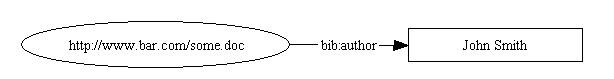
\includegraphics[scale=.50]{../immagini/RDFXML.jpg}
\caption{Rappresentazione grafica del grafo codificato nel listing \ref{esempioXML}}
\label{imgEsempioXML}
\end{figure}\newpage
Nell'esempio che segue è invece possibile notare come sfruttare uno statement come valore di una tripla:
\begin{lstlisting}[language=xml,firstnumber=1,caption={Esempio di metadato conforme ad RDF in XML},captionpos=b,label=esempioComplexXML]
<?namespace 
  href="http://docs.r.us.com/bibliography-info"
  as="bib"?> 
<?namespace href="http://www.w3.org/schemas/rdf-schema"
  as="RDF"?> 
<RDF:serialization> 
  <RDF:assertions href="http://www.bar.com/some.doc"> 
    <bib:author> 
      <RDF:resource> 
        <bib:name>John Smith</bib:name> 
        <bib:email>john@smith.com</bib:email> 
        <bib:phone>+1 (555) 123-4567</bib:phone> 
      </RDF:resource> 
    </bib:author> 
  </RDF:assertions> 
</RDF:serialization>
\end{lstlisting}
Risulta possibile anche ottenere una scrittura più modulare, sfruttando la proprietà \textit{id} del tag \textit{resource}:
\begin{lstlisting}[language=xml,firstnumber=1,caption={Esempio di metadato conforme ad RDF in XML},captionpos=b,label=esempioIdXML]
<?namespace href=
  "http://docs.r.us.com/bibliography-info" as="bib"?> 
<?namespace href=
  "http://www.w3.org/schemas/rdf-schema"as="RDF"?> 
<RDF:serialization> 
  <RDF:assertions href="http://www.bar.com/some.doc"> 
    <bib:author href="#John_Smith"/> 
  </RDF:assertions> 
</RDF:serialization>
<RDF:resource id="John_Smith"> 
  <bib:name>John Smith</bib:name> 
  <bib:email>john@smith.com</bib:email> 
  <bib:phone>+1 (555) 123-4567</bib:phone> 
</RDF:resource> 
\end{lstlisting}
Entrambi gli esempi mostrati nei listing \ref{esempioComplexXML} e \ref{esempioIdXML} hanno la seguente rappresentazione grafica:
\begin{figure}[H]
\centering
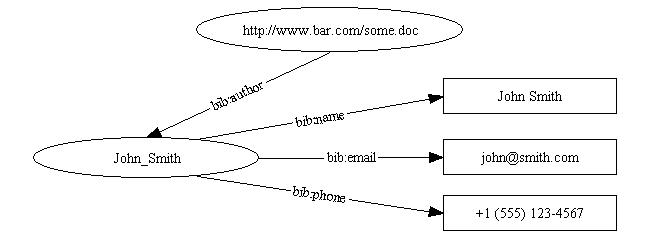
\includegraphics[scale=.50]{../immagini/complexXML.jpg}
\caption{Rappresentazione grafica del grafo codificato nei listing \ref{esempioComplexXML} e \ref{esempioIdXML}}
\label{imgEsempioComplexXML}
\end{figure}
\paragraph{Tag namespace}\mbox{}\\
Il tag \textit{namespace} è un'estensione alla specifica RDF attualmente non obbligatorio. Questo tag è stato introdotto per rendere la sintassi di un tag specifico al dominio applicativo meno prolissa:
\begin{itemize}
 \item \textbf{as}: proprietà del tag che indica il nome del namespace;
 \item \textbf{href}: porzione di identificativo da sostituire al valore della proprietà \textit{as} quando lo si incontra.
\end{itemize} 
Prendendo ad esempio il listing \ref{esempioComplexXML}: il tag \textit{bib:name} è da interpretare come: \\\url{http://docs.r.us.com/bibliography-info/name}\\ il valore così ottenuto risulta essere l'URI che identifica la proprietà; è anche un riferimento a dove è possibile recuperare informazioni su di essa.\\
L'utilizzo di questa pratica è diffuso anche in ODRL: nel listing \ref{esempioParty} il tag \textit{@context} svolge un ruolo simile: fa riferimento ad un file RDF nel quale sono definite tutte le abbreviazioni utili ad ODRL tramite le seguenti linee di codice:
\begin{lstlisting}[language=json,firstnumber=1,caption={Estratto context ODRL\cite{ODRLContext}},captionpos=b,label=contextJSONLD]
"odrl":       "http://www.w3.org/ns/odrl/2/",
"Permission": "odrl:Permission",
"permission": {"@type": "@id", "@id": "odrl:permission"}
\end{lstlisting}
Il formato di serializzazione utilizzato nel listing \ref{contextJSONLD} non è XML, bensì JSON-LD, lo stesso utilizzato nei vari esempi presentati nel capitolo \ref{ODRLChapter} relativo ad ODRL.\\
All'interno del lavoro di tesi, le serializzazioni utilizzate sono:
\begin{itemize}
\item JSON-LD: utilizzato negli esempi ed in input al processo di merging;
\item Turtle\cite{Turtle}: utilizzato come output del processo di merging. Tale decisione è stata presa poiché risulta essere la serializzazione più matura supportata dal framework Jena.
\end{itemize}
\subsection{RDFS}
Come esposto in precedenza, il modello RDF fornisce la sintassi necessaria per creare metadati in grado di rappresentare relazioni tra le varie risorse, lasciando libertà assoluta sul significato che queste relazioni possono avere. RDFS è ``[...]un'estensione semantica''\cite{RDFS} di RDF che permette di descrivere gruppi di risorse correlate tra loro e le relazioni tra i vari gruppi. RDFS basa il suo funzionamento sulla definizione di due termini:
\begin{itemize}
\item \textbf{rdfs:Class}: raggruppamento di risorse con le stesse proprietà, come ad esempio la classe \textit{odrl:Policy};
\item \textbf{rdf:Property}: relazione tra risorse oggetto e risorse valore di una tripla; istanze di questa particolare classe possiedono a loro volta le seguenti proprietà:
\begin{itemize}
\item \textbf{rdfs:range}: i \textit{valori} in una tripla di questa \textit{Property} devono essere istanze delle classi specificate in questa proprietà;  
\item \textbf{rdfs:domain}: gli \textit{oggetti} in una tripla di questa \textit{Property} devono essere istanze delle classi specificate in questa proprietà.
\end{itemize}
\end{itemize}
\newpage
Oltre a quanto appena mostrato, esistono anche due proprietà denominate: \textbf{rdfs:subClassOf} e \textbf{rdfs:subPropertyOf}. Queste \textit{Property} permettono di definire un sistema di ereditarietà tra classi e tra proprietà; ad esempio nel vocabolario ODRL si ha:\\
\begin{lstlisting}[language=xml,firstnumber=1,caption={Estratto vocabolario ODRL\cite{ODRVocab}},captionpos=b,label=vocabExtract]
<rdfs:Class 
  rdf:about="http://www.w3.org/ns/odrl/2/Prohibition">
  
  <rdfs:isDefinedBy 
    rdf:resource="http://www.w3.org/ns/odrl/2/"/>
  
  <rdfs:label xml:lang="en">Prohibition</rdfs:label>
  <rdfs:subClassOf
   rdf:resource="http://www.w3.org/ns/odrl/2/Rule"/>
  
</rdfs:Class>
  \end{lstlisting}
L'esempio appena mostrato è la definizione della sottoclasse \textit{Prohibition}, esposta nella sezione \ref{ODRLRulePara}. Un secondo esempio, sempre visibile in ODRL, è la definizione della proprietà ``odrl:partOf'', mostrata nei listing \ref{esempioAssetColl} e \ref{esempioPartyColl}, che presenta:
\begin{itemize}
\item due possibili \textit{rdfs:domain} e due possibili \textit{rdfs:range};
\item solo due coppie \textit{rdfs:domain}-\textit{rdfs:range} sono valide; questa restrizione è espressa mediante OWL\cite{OWL}, ulteriore estensione semantica utilizzata per espriremere concetti logici complessi;
\item i valori possibili per queste proprietà sono le due classi \textit{odrl:Party} ed \textit{odrl:Asset}.
\end{itemize}
\subsection{Apache Jena}\label{apacheJenaSec}
``Apache Jena (o Jena) è un framework Java free ed open source per creare applicazioni del semantic web o che sfruttano Linked Data. Il framework è composto da diverse API che interagiscono al fine di processare dati RDF.''\cite{Jena}\\
Per questo motivo si è scelto Jena come insieme di utility sia a supporto della porzione di parsing, descritta nella sezione \ref{parsingSection}, sia a supporto della porzione di produzione del documento ODRL finale, descritta nella sezione \ref{produceSection}. Nel dettaglio, le API utilizzate comprendono:
\begin{itemize}
\item \textbf{Core RDF API};
\item \textbf{Jena schemagen};
\item \textbf{ARQ - A SPARQL Processor for Jena};
\item \textbf{Modulo I/O}.
\end{itemize}
\paragraph{Core RDF API}\mbox{}\\
Questa porzione del framework offre interfacce per l'interazione con il modello RDF. La rappresentazione offerta da questa libreria si basa su triple, i cui elementi sono denominati:
\begin{itemize}
\item \textbf{resource}: l'oggetto dello statement codificato dalla tripla;
\item \textbf{property}: il predicato dello statement;
\item \textbf{value}: il valore dello statement, il quale può essere a sua volta una risorsa.
\end{itemize}
L'interfaccia principale fornita da questo componente è denominata \textit{Model} e denota un intero grafo RDF. Questa interfaccia è utilizzata per operazioni con alto livello di astrazione sull'intero modello, come per esempio:
\begin{itemize}
\item specificare su quale file o collezione di file RDF sta lavorando;
\item aggiungere, recuperare e rimuovere nodi dal grafo;
\item settare i \textit{namespace} utilizzati all'interno del modello;
\item settare la serializzazione del modello;
\item interagire con l'API ARQ per interrogare il modello tramite query SPARQL.
\end{itemize}
\paragraph{Jena schemagen}\mbox{}\\
Questo tool ha utilità puramente tecnica, in quanto è uno strumento per ``[...]convertire vocabolari OWL o RDFS in una classe Java class che contiene costanti statiche per i termini nel vocabolario''.\\
L'effettivo utilizzo del tool si traduce nel processare un file RDF, in questo caso il file context di ODRL\cite{ODRLContext}, automatizzando il processo di estrazione dei termini all'interno del vocabolario. I vantaggi di questo approccio si traducono in:
\begin{itemize}
\item l'utilizzo di variabili facilmente leggibili all'interno del linguaggio ARQ, anziché dell'URI che definisce la classe o la proprietà;
\item un'interazione più trasparente con le \textit{Core RDF API} in fase di aggiunta risorse o di definizione delle proprietà di un nodo.
\end{itemize}
Il contributo di questo tool non è direttamente visibile all'interno del codice del progetto di tesi, poiché ne è stata sfruttata la versione standalone.
\paragraph{ARQ e SPARQL}\mbox{}\\
``ARQ è il query engine fornito da Jena che supporta il linguaggio SPARQL RDF Query.''\cite{Jena}\\
Il linguaggio ``SPARQL può essere usato per esprimere query su diverse sorgenti di dati, sia su dati nativi RDF o esposti come RDF via middleware.''\cite{SPARQL}\\
L'obiettivo di queste tecnologie è fornire interfacce che permettano l'interrogazione di modelli RDF. ARQ è l'API esposta da Jena per formulare le interrogazioni tramite Java ; SPARQL è il linguaggio nel quale è espressa la query.\\
Prendendo ad esempio il seguente file in formato RDF:\\

\begin{lstlisting}[language=xml,firstnumber=1,caption={File sul quale si vuole eseguire una query},captionpos=b,label=SPARQLRDF]
@prefix dc:   <http://purl.org/dc/elements/1.1/> .
@prefix :     <http://example.org/book/> .
@prefix ns:   <http://example.org/ns#> .

:book1  dc:title  "SPARQL Tutorial" .
:book1  ns:price  42 .
:book2  dc:title  "The Semantic Web" .
:book2  ns:price  23 .

\end{lstlisting}
\begin{lstlisting}[language=sql,firstnumber=1,caption={Query SPARQL per il recupero dei titoli che iniziano per SPARQL},captionpos=b,label=SPARQLQuery]

PREFIX  dc:  <http://purl.org/dc/elements/1.1/>
SELECT  ?title
WHERE   { ?x dc:title ?title
          FILTER regex(?title, "^SPARQL") 
        }
\end{lstlisting}\mbox{}\\ \\  
Il risultato della query nel listing \ref{SPARQLQuery} è la tupla:
\begin{center} (\textbf{title} = ``SPARQL Tutorial'')\end{center}
\newpage
Questo secondo esempio mostra come sia possibile filtrare uno statement sulla base di più espressioni:\\
\begin{lstlisting}[language=sql,firstnumber=1,caption={File sul quale si vuole eseguire una query},captionpos=b,label=SPARQLRDF2]
@prefix foaf:  <http://xmlns.com/foaf/0.1/> .

_:a  foaf:name   "Johnny Lee Outlaw" .
_:a  foaf:mbox   <mailto:jlow@example.com> .
_:b  foaf:name   "Peter Goodguy" .
_:b  foaf:mbox   <mailto:peter@example.org> .
_:c  foaf:mbox   <mailto:carol@example.org> .
\end{lstlisting}\mbox{}

\begin{lstlisting}[language=sql,firstnumber=1,caption={Query SPARQL per il recupero dei nomi e delle mail solo per soggetti che presentano entrambe le proprietà},captionpos=b,label=SPARQLQuery2]
PREFIX foaf:   <http://xmlns.com/foaf/0.1/>
SELECT ?name ?mbox
WHERE
  { ?x foaf:name ?name .
    ?x foaf:mbox ?mbox }
\end{lstlisting}\mbox{}
Il risultato della query nel listing \ref{SPARQLQuery} sono le tuple:
\begin{center}
(\textbf{name} = "Johnny Lee Outlaw", \textbf{mbox} = <mailto:jlow@example.com>)\\
(\textbf{name} = "Peter Goodguy",	\textbf{mbox} = <mailto:peter@example.org>)
\end{center}
Risulta possibile notare che l'ultima tripla presente nel listing \ref{SPARQLRDF2} non sia stata utilizzata per costruire il risultato della query, poiché l'oggetto \textit{\_:c} non ha la proprietà \textit{foaf:name}.\\
Il ruolo che hanno le API ARQ all'interno di del progetto è di collegamente tra le query e le \textit{CORE RDF API}; introducono anche una semplificazione della sintassi evitando il costrutto \textit{PREFIX} dove è noto il modello sul quale si eseguono le query.
\newpage
\paragraph{Modulo I/O}\mbox{}
Il modulo Input/Output fornisce le interfacce necessarie:
\begin{itemize}
\item alla lettura di un file in formato RDF, supportando le serializzazioni:
\begin{itemize}
\item Turtle;
\item N-Triples;
\item N-Quads;
\item TriG;
\item RDF/XML;
\item JSON-LD;
\item RDF/JSON;
\item TriX;
\item RDF Binary;
\end{itemize}
\item alla scrittura di un file in formato RDF, supportando le medesime serializzazioni mostrate in lettura.
\end{itemize}
Il modello espresso mediante \textit{CORE RDF API} ottenuto da questi moduli è il medesimo a discapito della serializzazione utilizzata, di conseguenza non è necessario, almeno in lettura, attuare implementazioni specifiche basate sul formato. Quest'ultima constatazione vale anche per il procedimento di parsing e, quindi, per l'intera procedura di merging. L'unica porzione del progetto che necessita di adattamenti in base al formato risulta essere il produttore di documenti ODRL, in quanto alcuni formati possono necessitare di alcune modifiche per essere resi più leggibili dagli utenti finali. Non sono invece necessari adattamenti per l'utilizzo da parte di un programma.
\chapter{Valutazione casistiche}
\section{Casistiche di merging}
\paragraph{Casi base}
\subparagraph{Asset diffrenti}\mbox{}\\

\begin{lstlisting}[language=json,firstnumber=1,caption={La policy 1010 permette di riprodurre l'asset 9898.movie a chiunque},captionpos=b]
{
 "@context": "http://www.w3.org/ns/odrl.jsonld",
 "@type": "Set",
 "uid": "http://example.com/policy:1010",
 "permission": [{
   "target": "http://example.com/asset:9898.movie",
   "action": "play"
 }]
}

\end{lstlisting}


\begin{lstlisting}[language=json,firstnumber=1,caption={La policy 1011 consente la riproduzione dell'asset 1349.mp3 a chiunque},captionpos=b]
{
 "@context": "http://www.w3.org/ns/odrl.jsonld",
 "@type": "Set",
 "uid": "http://example.com/policy:1011",
 "permission": [{
   "target": "http://example.com/asset:1349.mp3",
   "action": "play"
 }]
}
\end{lstlisting}
Le due policy mostrate si riferiscono ad asset differenti, farne il merging porta semplicemente ad una policy avente entrambe le \textit{permission} già enunciate.
\subparagraph{Rule indipendenti}\mbox{}\\
\begin{lstlisting}[language=json,firstnumber=1,caption={La policy 1010 consente la riproduzione dell'asset 9898.movie a chiunque},captionpos=b]
{
 "@context": "http://www.w3.org/ns/odrl.jsonld",
 "@type": "Set",
 "uid": "http://example.com/policy:1010",
 "permission": [{
   "target": "http://example.com/asset:9898.movie",
   "action": "play"
 }]
}
\end{lstlisting}
\begin{lstlisting}[language=json,firstnumber=1,caption={La policy 1011 proibisce la distribuzione dell'asset 9898.movie a chiunque},captionpos=b]
{
 "@context": "http://www.w3.org/ns/odrl.jsonld",
 "@type": "Set",
 "uid": "http://example.com/policy:1011",
 "prohibition": [{
   "target": "http://example.com/asset:9898.movie",
   "action": "distribute"
 }]
}
\end{lstlisting}
Nonostante le due policy si riferiscano allo stesso asset anche in questo caso non è possibile combinare le due regole, poiché si riferiscono ad azioni tra loro scollegate. Un eventuale merging delle due policy avrebbe due regole distinte uguali a quelle di partenza.\newpage
\subparagraph{Attori designati differenti}\mbox{}\\
\begin{lstlisting}[language=json,firstnumber=1,caption={La policy 0001 permette un qualsiasi utilizzo dell'asset 1212 da parte del soggetto Billie},captionpos=b]
{
 "@context": "http://www.w3.org/ns/odrl.jsonld",
 "@type": "Policy",
 "uid": "http://example.com/policy:0001",
 "permission": [{
   "target": "http://example.com/asset:1212",
   "action": "use",
   "assigner": "http://example.com/owner:181",
   "assignee": 
	   "http://example.com/party:person:billie"
 }]
}
\end{lstlisting}
\begin{lstlisting}[language=json,firstnumber=1,caption={La policy 0002 proibisce la riproduzione dell'asset 1212 da parte del soggetto Alice},captionpos=b]
{
 "@context": "http://www.w3.org/ns/odrl.jsonld",
 "@type": "Policy",
 "uid": "http://example.com/policy:0002",
 "prohibition": [{
   "target": "http://example.com/asset:1212",
   "action": "play",
   "assigner": "http://example.com/owner:181",
   "assignee": 
        "http://example.com/party:person:alice"
 }]
}
\end{lstlisting}
In questo caso le regole espresse dalle due policy sarebbero in conflitto, poiché \textit{use}, permesso dalla prima policy, comprende al suo interno anche \textit{play}, proibito dalla seconda. Siccome però le due regole sono applicate a due soggetti diversi, un eventuale merging delle policy avrebbe due regole distinte uguali a quelle di partenza. Questa casistica non è stata ulteriormente esplorata all'interno del lavoro di tesi poiché:
\begin{itemize}
\item la procedura di merging implementata utilizza come semplificazione regole riferite ad \textbf{EveryOne}; questo perché il progetto MOSAICrOWN ha il suo focus sui dati;
\item un'eventuale procedura che tenga conto anche degli utenti aggiungerebbe solo un filtraggio preliminare sulle entità cui si riferiscono le regole.
\end{itemize}
\label{noStrat}
\paragraph{Conflitti senza strategia risolutiva indicata}\label{noStrat}\mbox{}\\
Nel caso due policy siano in conflitto quando non viene indicato alcun processo di risoluzione dei conflitti, ODRL invalida entrambe le policy. Attuando policy merging è possibile formulare una terza policy che racchiude entrambi i requisiti espressi dai documenti originali.
\subparagraph{Conflitti permesso-permesso}\label{permperm}\mbox{}\\
\begin{lstlisting}[language=json,firstnumber=1,caption={La policy 0001 permette un qualsiasi utilizzo dell'asset 1212 a chiunque},captionpos=b]
{
 "@context": "http://www.w3.org/ns/odrl.jsonld",
 "@type": "Policy",
 "uid": "http://example.com/policy:0001",
 "permission": [{
   "target": "http://example.com/asset:1212",
   "action": "play"
 }]
}
\end{lstlisting}
\begin{lstlisting}[language=json,firstnumber=1,caption={La policy 0002 permette la riproduzione dell'asset 1212 a chiunque},captionpos=b]
{
 "@context": "http://www.w3.org/ns/odrl.jsonld",
 "@type": "Policy",
 "uid": "http://example.com/policy:0002",
 "permission": [{
    "target": "http://example.com/asset:1212",
    "action": "display"
 }]
}
\end{lstlisting}
La seconda policy risulta in conflitto con la prima, poiché quest'ultima permette un numero maggiore di utilizzi. Seguendo la procedura standard, entrambe le due policy dovrebbero essere considerate non valide. Nella realtà dei fatti, facendo policy merging, si otterrebbe solamente la policy più restrittiva, ovvero la seconda. La procedura di policy merging in questione sarebbe quindi: 
\begin{enumerate}
	\item invalidare le policy 0001 e 0002;
	\item creare una terza policy 0003, uguale alla 0002 (la più restrittiva delle due), al fine di segnalare il processo di merging avvenuto.
\end{enumerate}
\subparagraph{Conflitti divieto-divieto}\label{divdiv}\mbox{}\\
\begin{lstlisting}[language=json,firstnumber=1,caption={La policy 0001 proibisce un qualsiasi utilizzo dell'asset 1212 a chiunque},captionpos=b]
{
 "@context": "http://www.w3.org/ns/odrl.jsonld",
 "@type": "Policy",
 "uid": "http://example.com/policy:0001",
 "prohibition": [{
    "target": "http://example.com/asset:1212",
    "action": "play"
 }]
}
\end{lstlisting}
\begin{lstlisting}[language=json,firstnumber=1,caption={La policy 0002 proibisce la riproduzione dell'asset 1212 a chiunque},captionpos=b]
{
 "@context": "http://www.w3.org/ns/odrl.jsonld",
 "@type": "Policy",
 "uid": "http://example.com/policy:0002",
 "prohibition": [{
    "target": "http://example.com/asset:1212",
    "action": "display"
 }]
}
\end{lstlisting}
Caso duale del precedente; in questo caso una delle due policy proibisce un numero maggiore di utilizzi rispetto all'altra. La procedura da seguire risulta essere:
\begin{enumerate}
	\item invalidare le policy 0001 e 0002;
	\item creare una terza policy 0003, uguale alla 0001(la più ampia delle due), al fine di segnalare il processo di merging avvenuto.
\end{enumerate}
\subparagraph{Conflitti permesso-divieto}\label{permdiv}\mbox{}\\
\begin{lstlisting}[language=json,firstnumber=1,caption={La policy 0001 permette il trasferimento dell'asset 1212 al soggetto Alice},captionpos=b]
{
 "@context": "http://www.w3.org/ns/odrl.jsonld",
 "@type": "Policy",
 "uid": "http://example.com/policy:0001",
 "permission": [{
   "target": "http://example.com/asset:1212",
   "assigner": "http://example.com/owner:181",
   "assignee": 
     "http://example.com/party:person:alice",
   "action": "transfer"
}]
}
\end{lstlisting}
\begin{lstlisting}[language=json,firstnumber=1,caption={La policy 0002 proibisce la vendita dell'asset 1212 al soggetto Alice},captionpos=b]
{
 "@context": "http://www.w3.org/ns/odrl.jsonld",
 "@type": "Policy",
 "uid": "http://example.com/policy:0002",
 "prohibition": [{
   "target": "http://example.com/asset:1212",
   "assigner": "http://example.com/owner:181",
   "assignee": 
     "http://example.com/party:person:alice",
   "action": "sell"
 }]
}
\end{lstlisting}
In questo caso, l'azione \textit{transfer} è inclusa in due sotto-azioni: \textit{give} e \textit{sell}; delle due sotto-azioni, solamente \textit{sell} è esplicitamente proibita dalla policy 0002, di conseguenza la seguente policy permette solo azioni che soddisfano entrambe le policy precedenti:\newpage
\begin{lstlisting}[language=json,firstnumber=1,caption={La policy 0003 consente al soggetto Alice di cedere l'asset 1212 senza richiedere un compenso e cancellando l'asset dal proprio insieme di dati},captionpos=b]
{
 "@context": "http://www.w3.org/ns/odrl.jsonld",
 "@type": "Policy",
 "uid": "http://example.com/policy:0002",
 "permission": [{
   "target": "http://example.com/asset:1212",
   "assigner": "http://example.com/owner:181",
   "assignee": 
     "http://example.com/party:person:alice",
   "action": "give"
 }]
}
\end{lstlisting}
Risulta possibile fare le seguenti valutazioni in merito a questa casistica:
\begin{itemize}
	\item il numero di regole all'interno della policy ottenuta per merging non è necessariamente minore rispetto al numero di regole di partenza;
	\item risulta necessario identificare se le sotto-azioni sono le uniche azioni atomiche possibili o se anche le azioni padre possano essere considerate atomiche; all'interno dell'implementazione è stata scelta la prima convenzione;
	\item se \textit{prohibition} e \textit{permission} fossero invertite tra la policy 0001 e la 0002, la policy 0003 risulterebbe una policy con solo divieti.
\end{itemize}
\paragraph{Conflitti con strategia risolutiva indicata}\mbox{}\\
Le strategie risolutive indicabili all'interno di ODRL utilizzando il Core Vocabulary sono le seguenti:
\begin{enumerate}
	\item \textit{perm}: tutte le \textit{permission} hanno la precedenza sulle \textit{prohibition};
	\item \textit{prohibit}: tutte le \textit{prohibition} hanno la precedenza sulle \textit{permission};
	\item \textit{invalid}: qualsiasi conflitto invalida la policy;
\end{enumerate}
La casistica \textit{invalid} è già stata trattata all'interno del paragrafo in sezione \ref{noStrat}. Per quanto concerne le altre due casistiche, come già esposto nella sezione \ref{problematicheSec}, lo standard ODRL risulta inadatto al trattamento di conflitti; questa proprietà viene quindi ignorata dal procedimento di merging.

\chapter{Implementazione}\label{implementazioniCh}
\section{Architettura generale}
\begin{figure}[htp]
\centering
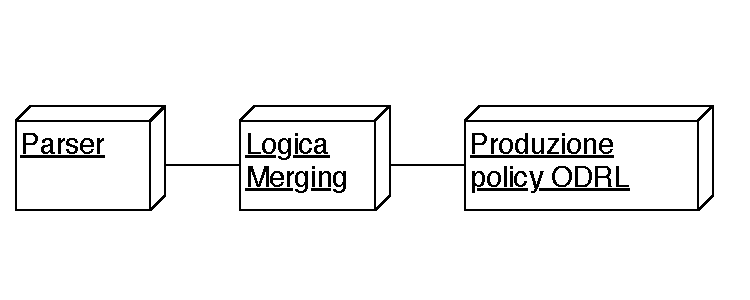
\includegraphics[scale=1]{../immagini/arch_gen.pdf}
\caption{Pipeline dei macro componenti della soluzione}
\label{archGenImpl}
\end{figure}
L'architettura generale è una semplice pipeline di componenti: il processo implementato risulta essere una serie di estrazioni di dati dai documenti ODRL in ingresso. L'output ottenuto ha le seguenti proprietà:
\begin{itemize}
\item è il risultato dell'unione o dell'intersezione delle policy in ingresso;
\item esprime le regole in un formato non ambiguo per l'interrogazione puntuale.
\end{itemize}
Queste processo viene attuato all'interno del componente denominato \textit{Logica Merging}, il quale si occupa di aggiungere la semantica necessaria al modello ODRL.\\
Il primo componente della pipeline si occupa di estrarre le informazioni di rilievo dalle policy in ingresso mentre il componente in coda ha il ruolo di produttore di documenti conformi ad ODRL.
\section{Parser}\label{parsingSection}
Il primo componente della pipeline è il parser di documenti ODRL. Il suo ruolo è estrarre le informazioni utili alla procedura di merging. Questo componente sfrutta il framework Apache Jena esposto nella sezione \ref{apacheJenaSec}. Le interfacce esposte da questa porzione della soluzione sono:
\begin{itemize}
\item un'interfaccia per il recupero delle \textit{Rule} relative ad ogni \textit{Asset} all'interno della policy;
\item un'interfaccia per il recupero delle relazioni \textit{partOf} tra i vari \textit{Asset} all'interno della policy.
\end{itemize}
La componentizzazione è stata fatta al fine di incapsulare al meglio queste due funzionalità, permettendone l'uso atomico qualora necessario. L'architettura del componente è mostrata nella seguente figura:
\begin{figure}[H]
\centering
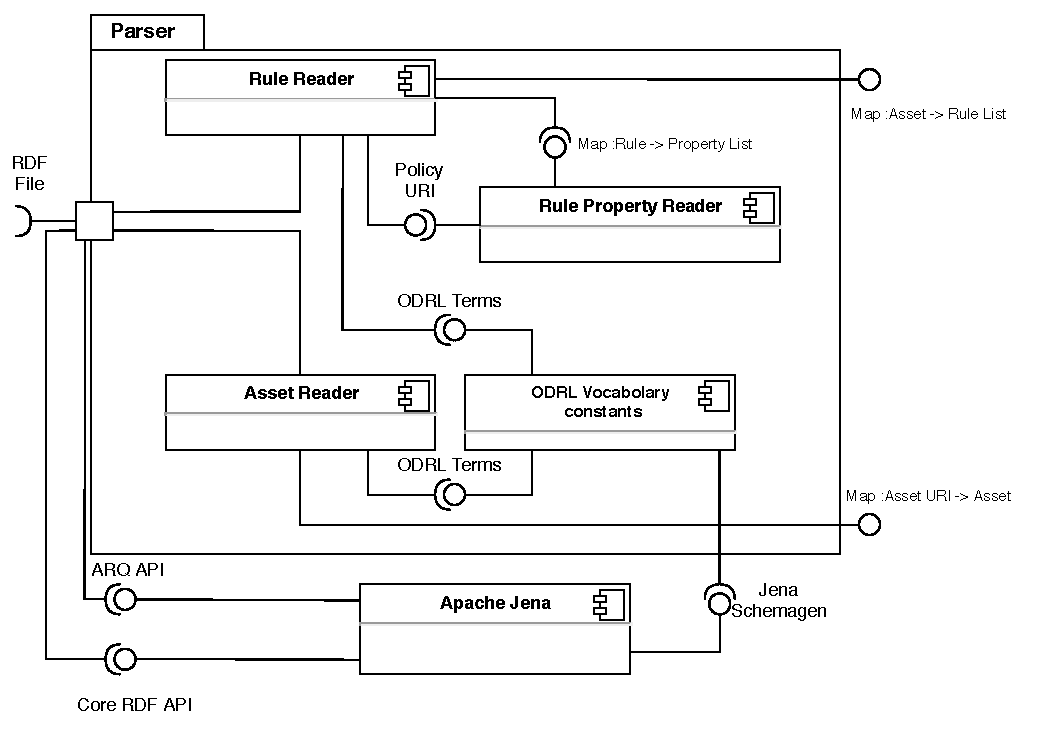
\includegraphics[scale=.80]{../immagini/parserDiagram.pdf}
\caption{Diagramma delle componenti per il parsing di documenti ODRL}
\label{parserUML}
\end{figure}
\subsection{Rule Reader}
Questo componente ha il ruolo di estrarre le regole presenti in una policy ed organizzarle in una mappa avente come chiavi gli \textit{Asset} e come valori le liste delle regole che hanno la chiave come \textit{target}. Il procedimento per la creazione della mappa segue i seguenti passi:
\begin{enumerate}
\item recupero degli URI delle singole policy contenute nel documento ODRL;
\item recupero della lista delle proprietà all'interno di una regola ODRL;
\item estrazione della proprietà \textit{target} dalle regole per popolare le chiavi della mappa;
\item estrazione delle proprietà \textit{type} e \textit{action} per creare il wrapper di una regola ODRL;
\item inserimento del wrapper all'interno della lista del rispettivo target.
\end{enumerate} 
Il primo passo della procedura è attuato grazie alla seguente query SPARQL:
\begin{lstlisting}[language=sql,firstnumber=1,caption={Query per il recupero dei dati relativi a tutte le policy contenute nel documento ODRL},captionpos=b]
SELECT *  WHERE {?policy <rdf:type> <odrl:Policy> .}
\end{lstlisting}
In questo modo è possibile identificare più policy all'interno del documento ODRL. L'URI delle varie policy è contenuto nel valore con chiave \textbf{policy} nelle tuple recuperate dalla query.\\
Il secondo passo della procedura è attuato mediante quest'ulteriore query SPARQL:
\begin{lstlisting}[language=sql,firstnumber=1,caption={Query per il recupero delle proprietà di tutte le regole},captionpos=b]
SELECT ?rule ?pred ?ogg ?type
WHERE {
	?policy ?type ?rule .
	?rule ?pred ?ogg
	FILTER (
		?type IN (<odrl:permission>,
		          <odrl:prohibition> )
		)
}
\end{lstlisting}
Le tuple recuperate hanno la seguente struttura:
\begin{itemize}
\item \textbf{rule}: uri autogenerato da ARQ per le regole, in quanto prive di URI nelle policy;
\item \textbf{pred}: proprietà all'interno della regola, per esempio \textit{odrl:action} o \textit{odrl:target};
\item \textbf{ogg}: valore della proprietà identificata dalla chiave \textit{pred};
\item \textbf{type}: valore delle proprietà \textit{rdf:type} della regola; come è possibile notare dalla clausola \textit{FILTER} può assumere solo i valori \textit{odrl:permission} o \textit{odrl:prohibition}.
\end{itemize}
Il risultato viene riorganizzato in una mappa che lega ogni regola ad una coppia \textit{proprietà-valore}.\\
Gli ultimi passi della procedura sono eseguiti analizzando la mappa ottenuta tramite il seguente algoritmo:
\begin{lstlisting}[language=java,firstnumber=1,caption={Pseudo codice per il popolamento della mappa finale},captionpos=b,label=parserRuleCode]
Map<Asset,List<Rule> mapAssetRuleList;
Iterator itRule = mappaParams.entrySet().iterator();

//Iterazione sulla mappa precedente
while(itRule.hasNext() ){

    MapEntry singleRule = itRule.next();
    List<Pair<String,String>> propertyList = singleRule.getValue();
    
    //Possibili property
    Asset collection = new Asset("EveryAsset");
    Action action = null;
    String type = "";
    
    //Itero per recuperare il valore delle varie property
	for(Pair<String,String> actProperty : propertyList){

	 if(actProperty == odrl:permission)
          type = "Permission";
	 if(actProperty == odrl:prohibition)
          type = "Prohibition";
	 if(actProperty == odrl:target)
          collection = new Asset(actProperty.Value);
	 if(actProperty == odrl:action)
	      action = actProperty.Value;
	}
	
    //Creazione del wrapper
    if(type.equals("Permission")
          rule = new Permission(action)
    else
          rule = new Prohibition(action)
    //Assegnazione wrapper a chiave corretta
    if(mapAssetRuleList.hasKey(collection){
          mapAssetRuleList.get(collection).add(rule);     
    }else{
          List<Rule> assetRuleList = new List();
          assetRuleList.add(rule);
          mapAssetRuleList.put(collection,assetRuleList);
    }
    resetTmp(collection,action,type);

}
return mapAssetRuleList;
\end{lstlisting}
Il codice mostrato nel listing \ref{parserRuleCode} risulta avere complessità lineare proporzionale al numero di proprietà recuperate dalle query SPARQL.
\subsection{Asset Reader}
Questo componente ha il ruolo di estrarre ogni asset presente nella policy che soddisfi almeno una delle seguenti condizioni:
\begin{itemize}
\item è il target di almeno una regola;
\item è il valore della proprietà \textit{partOf} di almeno un altro asset.
\end{itemize}
Tutti gli asset che non soddisfano almeno una di queste condizioni non sono utili alla procedura di merging, poiché non sono effettivamente regolamentati dalla policy ODRL e non portano informazioni di ereditarietà tra gli asset. Gli asset recuperati vengono poi organizzati in una mappa che collega il loro URI al wrapper utilizzato dalla procedura di merging. I wrapper sono creati con  le informazioni relative a legami di ereditarietà tra asset.\\
I passi per fornire questa funzionalità sono:
\begin{enumerate}
\item recupero di tutti gli asset presenti nella policy tramite query SPARQL che filtra le due proprietà citate precedentemente;
\item creazione dei wrapper ed inserimento all'interno della mappa che viene restituita come risultato finale;
\item per ogni asset, si esegue una query SPARQL che recupera tutti gli asset che lo hanno come parent;
\item si aggiorna ogni wrapper con l'informazione ottenuta dal passo precedente. 
\end{enumerate}
Di seguito la prima delle due query SPARQL effettuate:
\begin{lstlisting}[language=sql,firstnumber=1,caption={Query SPARQL per il recupero degli asset utili alla procedura di merging},captionpos=b,label=parserRuleCode]
SELECT DISTINCT ?obj  WHERE {
  ?sub ?pred ?obj
     FILTER (?pred IN
              (<odrl:target>, <odrl:partOf> )
            ) 
}
\end{lstlisting}
Le tuple restituite da questa query presentano come valore con chiave \textit{obj} l'URI degli asset che almeno una volta sono il valore di una proprietà \textit{odrl:target} o \textit{odrl:partOf}.\\
La seconda query necessaria al procedimento invece è la seguente:
\begin{lstlisting}[language=sql,firstnumber=1,caption={Query SPARQL per il recupero degli asset utili alla procedura di merging},captionpos=b,label=parserRuleCode]
SELECT DISTINCT ?sub  WHERE {
   ?sub <odrl:partOf> <parentURI>}
}
\end{lstlisting}
In questo caso le tuple restituite presentano come valore con chiave \textit{sub} l'URI degli asset che hanno la proprietà \textit{odrl:partOf} valorizzata con l'URI \textit{parentURI}: l'identificatore dell'asset per cui si sta iterando nel terzo passo della procedura.\\
Per ogni URI recuperato da questa query, si aggiorna il relativo wrapper aggiungendo alla lista dei parent il nodo dell'iterazione corrente.
\section{Logica Merging}
All'interno di questo componente sono implementate le funzionalità necessarie per l'effettivo merging delle policy in ingresso.\\
Le operazioni di merging che si punta a supportare sono di due tipi:
\begin{itemize}
\item \textbf{unione}: utilizzata all'iterno di uno scenario collaborativo; i permessi espressi da almeno una delle due policy rimangono validi nella policy output;
\item \textbf{intersezione}: utilizzata in uno scenario non collaborativo; un permesso appare nella policy in output solo se espresso all'interno di entrambi gli ingressi.
\end{itemize}
\subsection{Rappresentazione delle Azioni}\label{enumAction}
Uno dei fondamenti dell'implementazione sono le \textbf{Action}, ovvero gli utilizzi dell'asset regolabili dalle policy ODRL. Per rappresentarle si è utilizzato un enumerativo con la struttura mostrata in figura \ref{imgActionEnum}:
\begin{figure}[H]
\centering
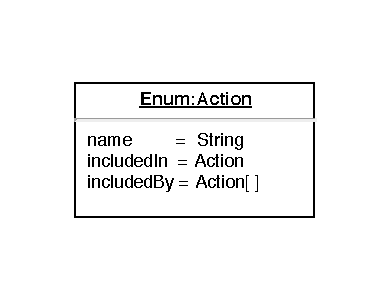
\includegraphics[scale=1.00]{../immagini/enumAction}
\caption{Struttura dell'enumerativo Action}
\label{imgActionEnum}
\end{figure}
All'interno dell'enumerativo è presente il nome che ha all'interno dell' ODRL Common Vocabulary, la lista delle azioni figlie e l'azione padre se esiste. Questa struttura è assimilabile a quella di un nodo in una struttura ad albero. L'enumerativo è provvisto dei metodi \textit{get} per il recupero delle informazioni presentate.
\subsection{Rappresentazione delle Regole}\label{ruleRappr}
Il secondo focus principale dell'implementazione sono le \textbf{Rule}, il cui stato all'interno della policy è gestito mediante un albero di regole. Questo è reso possibile sfruttando le relazioni tra le azioni espresse mediante l'enumerativo definito in figura \ref{imgActionEnum}. Per ottenere un maggior incapsulamento delle funzioni si è deciso di dividere la logica della struttura ad albero in due compenenti:
\begin{itemize}
\item il gestore dell'albero delle regole: questa componente si occupa delle azioni ad alta astrazione sull'albero delle regole come ad esempio il recupero di un nodo specifico, il settaggio di stato di un nodo, oppure il recupero dello stato di una regola;
\item il gestore del singolo nodo: questo componente si occupa dell'effetiva gestione del nodo rappresentante una regola; implementa operazioni come ad esempio il recupero del nodo padre o dei nodi figli; le funzionalità principali riguardano la propagazione di eventuali divieti lungo la gerarchia delle regole, sia verso i nodi figli che verso il nodo padre.
\end{itemize}
\begin{figure}[H]
\centering
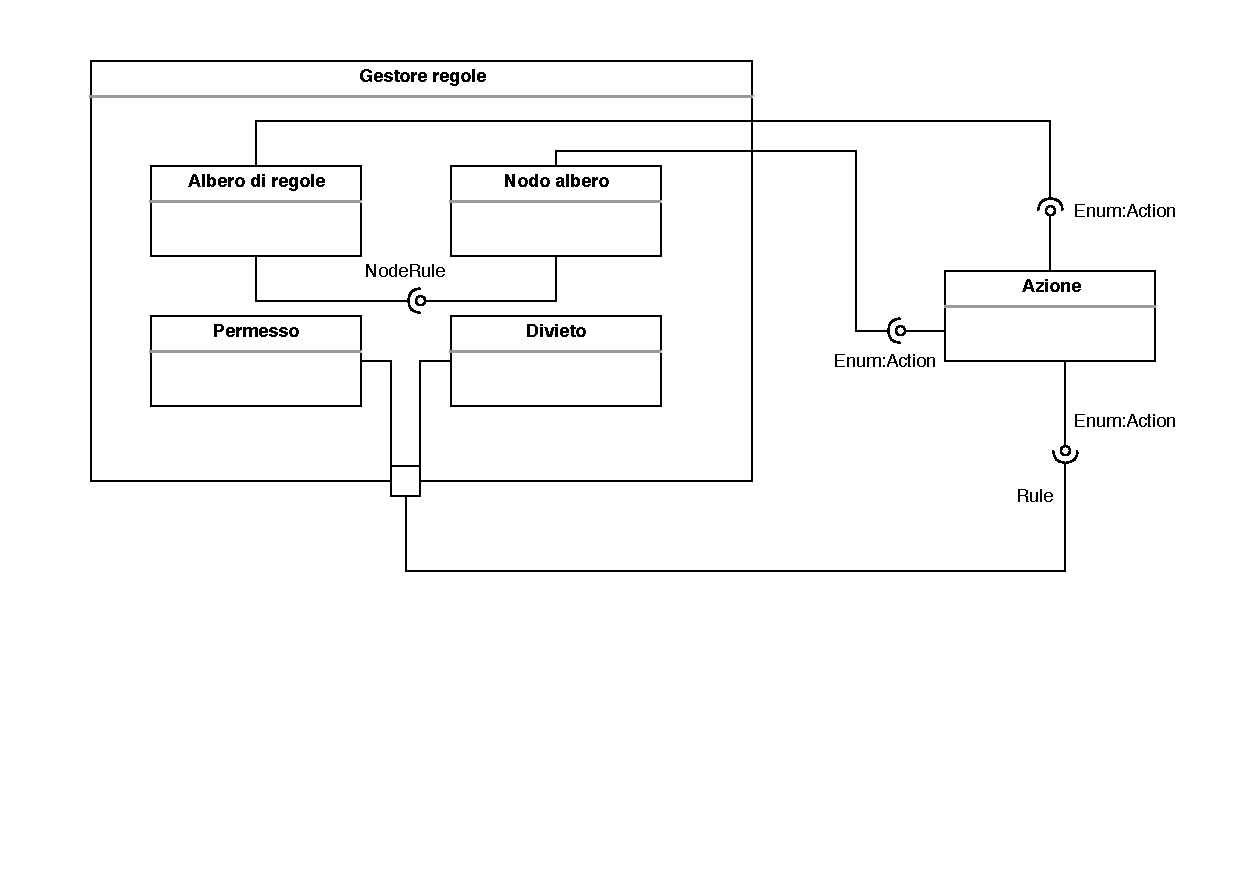
\includegraphics[scale=.60]{../immagini/imgCompRule}
\caption{Diagramma dei componenti per la rappresentazione delle regole}
\label{imgCompRule}
\end{figure}
Oltre ai componenti sopracitati in figura \ref{imgCompRule} è possibile vedere le implementazioni dell'interfaccia \textbf{Rule}, utilizzata anche per comunicare con il wrapper di policy.
\paragraph{Creazione dell'albero}\mbox{}\\
L'albero viene creato mediante un gestore apposito specificandone l'azione radice. Come esposto nella sezione \ref{enumAction}, l'enumerativo \textbf{Action} permette il recupero della lista delle azioni incluse dalla radice e quindi la creazione di eventuali sottoalberi. La creazione dei nodi figli è demandata al gestore del singolo nodo dell'albero.\\
Prendendo ad esempio l'azione \textbf{use} l'albero creato avrebbe la struttura seguente:
\begin{itemize}
\item il nodo relativo all'azione \textbf{use} è la radice dell'albero;
\item tutte le azioni incluse da \textbf{use} compongono il livello successivo;
\item le azioni che a loro volta ne includono altre, come ad esempio \textbf{play}, sono le radici del sottoalbero corrispondente alla loro gerarchia;
\item l'albero ha una struttura piatta, questo perché un'azione generica tende ad avere molti figli ma le azioni più specifiche tendono a non avere figli a loro volta.
\end{itemize}
\paragraph{Gestione dello stato di un'azione}\mbox{}\\
\label{ruleTree}
Ogni nodo dell'albero creato si riferisce ad una azione che può essere regolata e, oltre a tener conto della struttura gerarchica tra le azioni, rappresenta se l'azione si possa svolgere o meno. Gli stati in cui si può trovare un nodo sono tre:
\begin{enumerate}
\item \textbf{Permitted}: l'azione nel nodo è permessa esplicitamente;
\item \textbf{Prohibited}: l'azione nel nodo è proibita esplicitamente oppure tutte le sue azioni figlie sono nello stato \textbf{Prohibited}\footnote{Questa procedura è attuata tenendo conto dell'assunzione che azioni generiche non siano attuabili. Risulta possibile adattare l'approccio ad altre ipotesi.};
\item \textbf{Undefined}: l'azione nel nodo non ha regole che la interessano oppure almeno una azione figlia è \textbf{Prohibited} o \textbf{Undefined}.
\end{enumerate}
I singoli nodi si occupano anche di trasmettere lungo l'albero le conseguenze di un determinato cambio di stato:
\begin{enumerate}
\item settaggio a \textbf{Permitted}: il cambiamento viene propagato a tutti i nodi figli, a meno che:
\begin{itemize}
\item il nodo non fosse già nello stato \textbf{Prohibited}, in questo caso nessun settaggio viene svolto;
\item almeno uno dei nodi figli fosse nello stato \textbf{Prohibited} o \textbf{Undefined}, in questo caso il nodo rimane  \textbf{Undefined}, mentre sui nodi figli si attua il settaggio a \textbf{Permitted}.
\item il caso precedente si attua anche qualora uno dei nodi figli fosse \textbf{Undefined}.
\end{itemize}
\item settaggio a \textbf{Prohibited}: il cambiamento viene propagato a tutti i nodi figli. Inoltre il nodo padre viene settato come \textbf{Undefined} se almeno un altro figlio non è ancora stato vietato, altrimenti anche il padre è settato come \textbf{Prohibited}. La procedura attuata sul nodo padre è propagata fino alla radice della gerarchia;
\item settaggio a \textbf{Undefined}: questo settaggio avviene solamente come propagazione dai nodi figli nella casistica in cui non è necessario salire ulteriormente di livello.
\end{enumerate}
Di seguito alcuni esempi delle varie casistiche:
\begin{figure}[H]
\centering
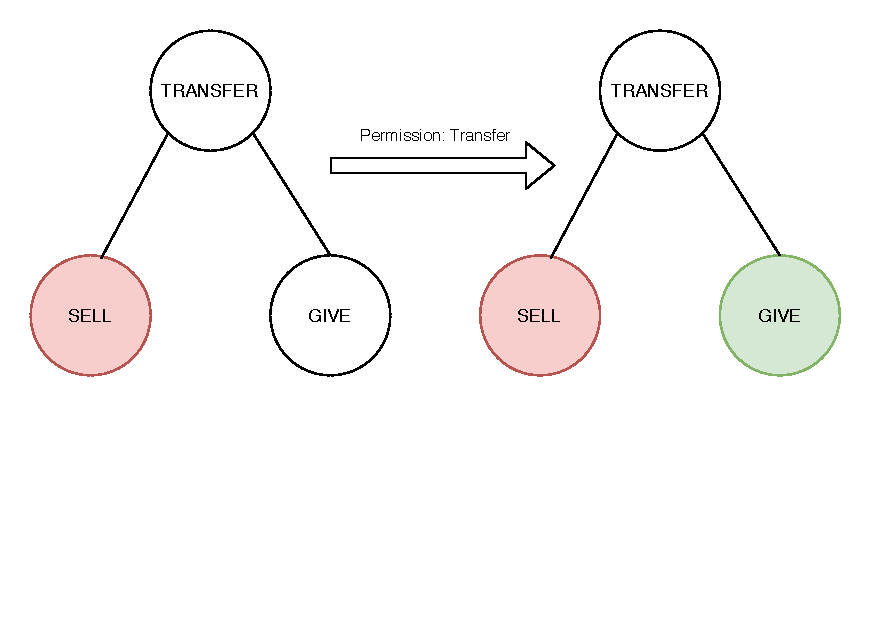
\includegraphics[scale=.50]{../immagini/propagationPerm}
\caption{Esempio di propagazione di un permesso, con azione figlia proibita}
\label{examplePerm}
\end{figure}
\begin{figure}[htp]
\centering
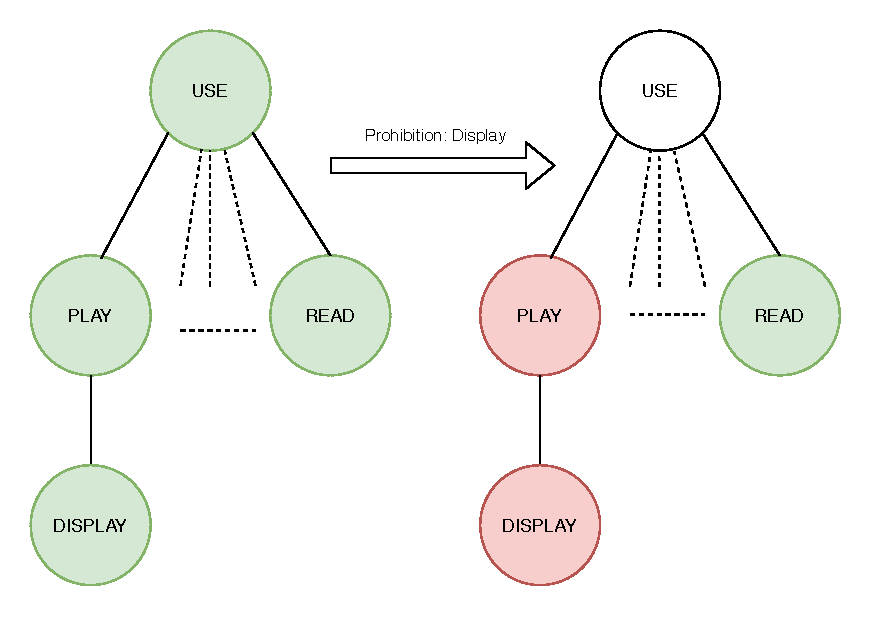
\includegraphics[scale=.50]{../immagini/propagationProParent}
\caption{Esempio di propagazione verso il padre di un divieto}
\label{exampleProParent}
\end{figure}

\paragraph{Recupero di un nodo e del suo stato}\mbox{}\\
L'albero creato non è binario e, di conseguenza, non supporta una ricerca efficiente dei nodi. Grazie alla gerarchia delle \textbf{Action} si ha un'alternativa efficiente: sfruttando l'enumerativo in figura \ref{imgActionEnum} è possibile ricostruire il percorso da un nodo foglia alla radice. Di seguito lo pseudo codice utilizzato per recuperare il nodo relativo ad un'azione:\\

\begin{lstlisting}[language=java,firstnumber=1,caption={Il caso peggiore per questa ricerca è la profondità della gerarchia delle azioni. Il caso migliore si ha qundo l'azione non è nell'albero, con tempo di risposta costante.},label=listingAlgoNode,captionpos=b]
public Node getActionNode(Action a){
List steps = [];
Action visited = a;
Node exploredNode = Tree.getRoot();

while(visited != None){
  steps.add(visited);
  visited = visited.getFatherAction();
}

// Sempre vero a meno che non si chiami
// il metodo su un albero con radice errata
if(exploredNode.getAction() == steps.getLastStep()){
  steps.popLast();
  while(!(exploredNode.getAction() == a)){
  	exploredNode=
  	   visitedNode.getChildsMap()
  	     .get(steps.getLastStep);
  	steps.popLast();
  }
else{
  // Caso di albero con radice errata
  return null; 
}

return exploredNode;
                
}
\end{lstlisting}
Per il recupero dello stato relativo ad una azione si usa il medesimo algoritmo mostrato nel listing \ref{listingAlgoNode} con un'ottimizzazione: se una delle azioni più in alto nella gerarchia si trova nello stato \textbf{Prohibited} o \textbf{Permitted} si ritorna quello stato e si interrompe la ricerca del nodo. Questa ottimizzazione è possibile poiché:
\begin{itemize}
\item se l'azione più in alto nella gerarchia è \textbf{Permitted}, necessariamente tutte le azioni nel suo sottoalbero sono \textbf{Permitted}; in caso contrario la radice del sottoalbero sarebbe \textbf{Undefined} o \textbf{Prohibited};
\item  se l'azione più in alto nella gerarchia è \textbf{Prohibited}, ogni azione nel suo sottoalbero è \textbf{Prohibited}.
\end{itemize}
Le prestazioni nel caso peggiore rimangono comunque dipendenti dalla profondità della gerarchia delle azioni, mentre tra i casi migliori si aggiunge lo scenario in cui l'azione radice dell'albero è \textbf{Prohibited} o \textbf{Permitted}: questa casistica ha tempo d'esecuzione costante.
\subsection{Rappresentazione Policy}\label{policyRappr}
Questa componente implementa le seguenti logiche:
\begin{itemize}
\item assegna agli asset target un insieme di regole;
\item le regole assegnate vengono rappresentate tramite 2 alberi delle regole: uno con radice \textbf{USE} ed uno con radice \textbf{TRANSFER};
\item si occupa di attuare il merging di 2 insiemi di regole;
\item le modalità di merging sono \textbf{intersect} e \textbf{union}.
\end{itemize}
\paragraph{Unione di policy}\mbox{}\\
L'unione di policy è un'operazione creata per supportare uno scenario collaborativo. All'interno di questo ambiente i permessi definiti da un attore vengono condivisi anche dall'altro. L'operazione è attuata eseguendo i seguenti passi:
\begin{enumerate}
\item unione della lisa delle regole tra delle policy in input;
\item creazione di una nuova policy avente il set di regole ottenuto al passo precedente;
\item la policy finale creata sfrutta la logica già esposta nel paragrafo \ref{ruleTree} per la gestione degli alberi delle regole.
\end{enumerate}
\paragraph{Intersezione di policy}\mbox{}\\
L'intersezione di policy è un'operazione creata per supportare uno scenario non collaborativo. In questo ambiente un attore non ha controllo sui permessi definiti da altre entità. In questo scenario un permesso è mantenuto solo nel caso in cui sia definito da entrambe le policy. La logica è attuata mediante i seguenti passi:
\begin{enumerate}
\item si recuperano gli stati relativi ad ogni azione in entrambe le policy; gli stati sono mantenuti in mappe aventi come chiave l'azione regolata; questo passo è attuato su entrambi gli input;
\item si itera sulle chiavi delle mappe e si effettuano i seguenti controlli:
\begin{itemize}
\item se l'azione è \textbf{Prohibited} in almeno una delle policy, si inserisce il divieto relativo tra le regole finali;
\item se l'azione è \textbf{Undefined} in almeno una delle policy, la si lascia non regolata;
\item se non si è nei due casi precedenti, l'azione allora è \textbf{Permitted} da entrambe e si inserisce il relativo permesso tra le regole finali;
\end{itemize}
\item si crea una nuova policy avente il set delle regole ottenuto grazie ai passi precedenti;
\item la policy finale creata sfrutta la logica già esposta nel paragrafo \ref{ruleTree} per la gestione degli alberi delle regole.
\end{enumerate}
\subsection{Rappresentazione Asset}\label{assetFun}
Questo componente implementa funzionalità relative alla gestione degli asset, le quali prevedono:
\begin{itemize}
\item supporto alla gerarchia degli asset, dando modo di esplicitare la proprietà \textbf{partOf};
\item collega un asset alla policy con regole che lo interessano;
\item propaga le regole di un asset alle collezioni figlie. Le possibili modalità di merging sono \textbf{intersect} ed \textbf{union}, esposte in sezione \ref{policyRappr}. Viene anche data la possibilità di non propragare la policy alle risorse figlie.
\end{itemize}
Per effetturare queste operazioni è stata usata un'architettura simile a quella mostrata nella sezione \ref{ruleRappr}; nel caso precedente sono state separate le funzionalità a livello di gerarchia da quelle relative al singolo nodo. Di seguito il diagramma delle componenti di questa sezione:
\begin{figure}[H]
\centering
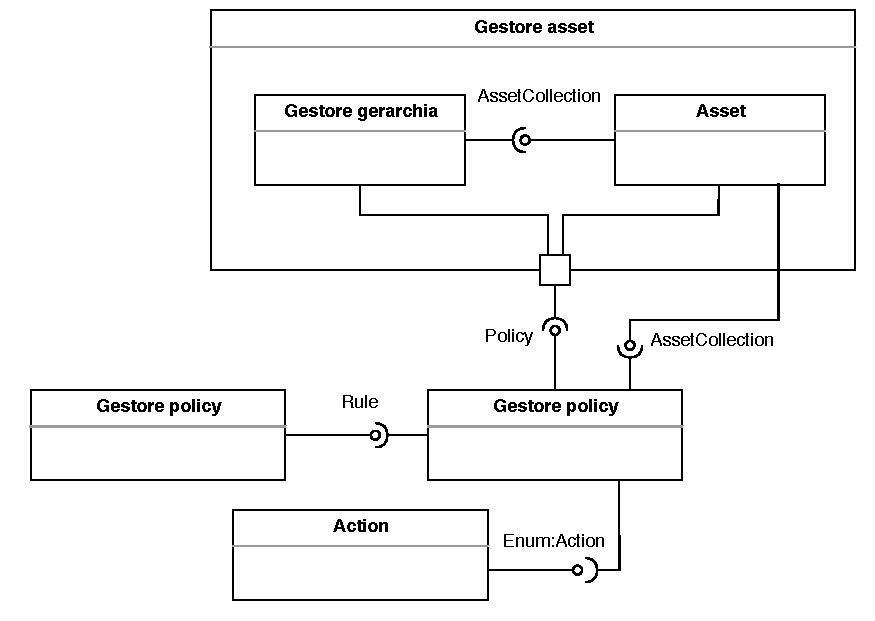
\includegraphics[scale=.7]{../immagini/compAsset.pdf}
\caption{Diagramma dei componenti per la rappresentazione degli asset}
\label{compAssetImg}
\end{figure}
Come è possibile notare dalla figura \ref{compAssetImg} questo componente sfrutta tutte le parti esposte in precedenza.\\
Lo scenario di utilizzo di un \textbf{Asset} si compone delle seguenti fasi:
\begin{enumerate}
\item definizione dei legami di gerarchia degli asset, tramite lettura della proprietà \textbf{partOf};
\item definizione delle regole relative all'asset e creazione della relativa policy;
\item assegnazione della policy al gestore della gerarchia degli asset;
\item il gestore si occupa di settare la policy per il nodo interessato e propagarla ai figli secondo la modalità indicata.
\end{enumerate}
\paragraph{Propagazione delle policy}\label{propagation}\mbox{}\\
La propagazione di una policy avviene dopo che questa è stata settata dal gestore della gerarchia degli asset. Il gestore si occupa quindi il nodo interessato dalla policy; per questa prima operazione si utilizza una ricerca in profondità data la natura ricorsiva dell'operazione di propagazione. Un'alternativa possibile è l'utilizzo di una ricerca in ampiezza, mantenendo il medesimo caso peggiore data l'assenza di cicli.\\
Dopo il recupero del nodo interessato dalla policy, si attua l'effettiva propagazione ad ogni nodo figlio, fino ad arrivare alle foglie. Per nodi senza policy, viene settata quella del nodo padre.\\
Di seguito alcuni esempi:
\begin{figure}[H]
\centering
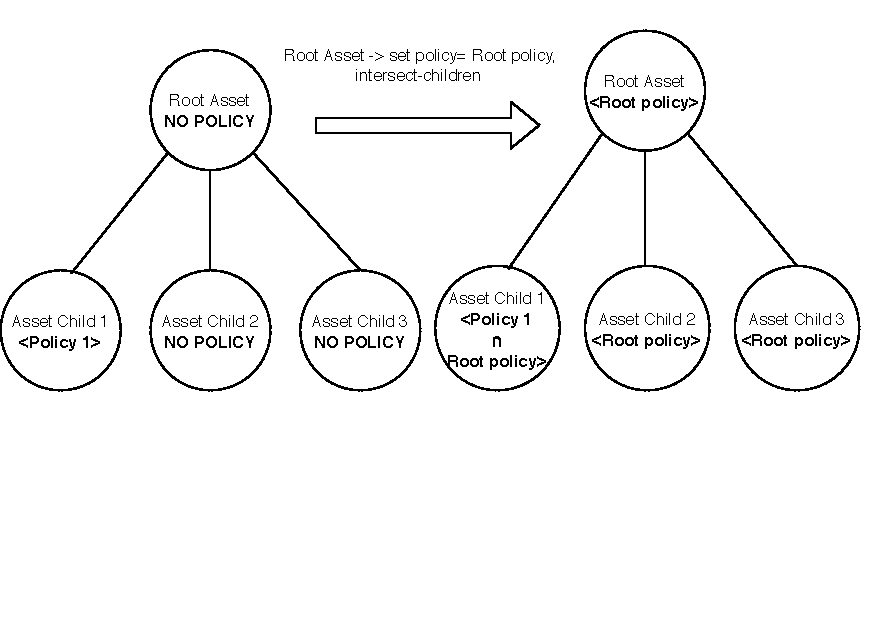
\includegraphics[scale=.65]{../immagini/assetSetPropagation.pdf}
\caption{Esempio di propagazione di una policy quando l'asset padre non ha policy, modalità con intersezione}
\label{imgAssetPropSet}
\end{figure}
\begin{figure}[H]
\centering
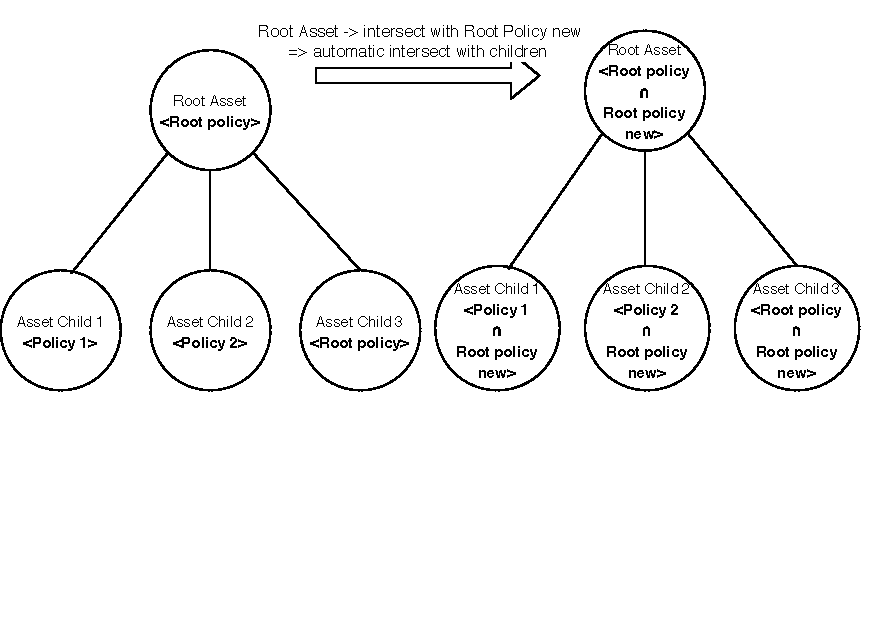
\includegraphics[scale=.65]{../immagini/assetIntersectPropagation.pdf}
\caption{Esempio di propagazione di una intersezione di policy}
\label{imgAssetPropIntersect}
\end{figure}
Un processo analogo a quanto mostrato nelle figure \ref{imgAssetPropSet} e \ref{imgAssetPropIntersect} può sfruttare anche operazioni di unione. nella figura \ref{imgAssetPropIntersect} è possibile notare che se un asset figlio non ha una policy eredita in modo completo quella del nodo padre.
\paragraph{Recupero policy in seguito alla propagazione}\label{recuperoPolicy}\mbox{}\\
La policy relativa ad un nodo ai livelli più bassi può cambiare drasticamente in seguito ad una operazione di propagazione, come mostrato nelle figure \ref{imgAssetPropSet} e \ref{imgAssetPropIntersect}. Il gestore della gerarchia degli asset implementa una procedura di recupero policy di uno specifico nodo: si percorre in ampiezza l'intera gerarchia, recuperando ogni policy. Questa procedura restituisce una mappa che collega l'URI di ogni risorsa nella gerarchia alla sua policy. nel set di chiavi sono presenti anche i nodi non aventi una policy.
\subsection{Gestore procedura di merging}
Tutte le componenti fino ad ora mostrate si concentrano in modo atomico su una singola porzione della procedura di merging, supportando operazioni di intersezione ed unione. Tutte le componenti lavorano però su un singolo documento ODRL. Il componente mostrato in questa sezione si occupa di supervisionare l'intera procedura. Di seguito il diagramma delle componenti che interessano il processo:
\begin{figure}[H]
	\centering
	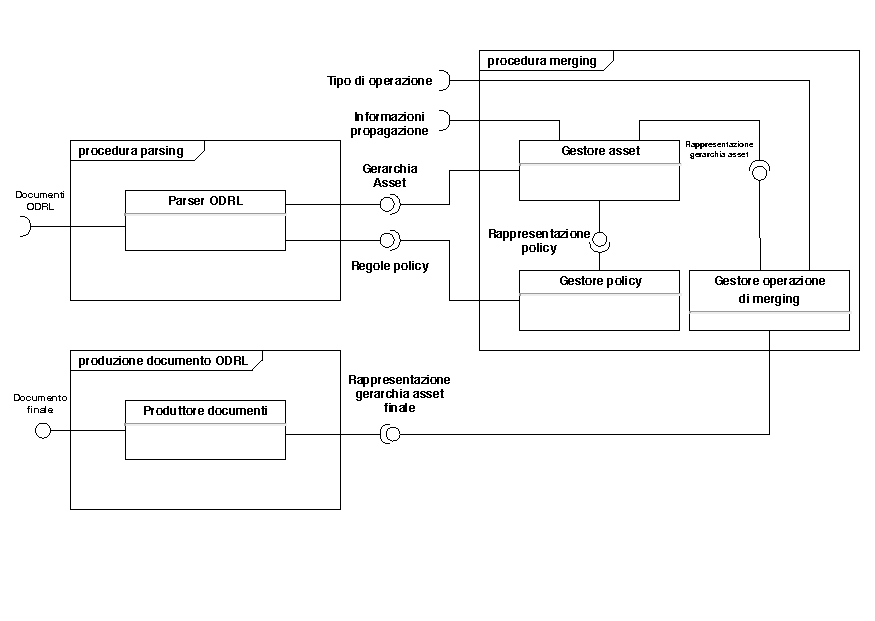
\includegraphics[scale=.70]{../immagini/processoMergin.pdf}
	\caption{Componenti che interagiscono nel processo di merging di policy ODRL}
	\label{procMergin}
\end{figure}
Dalle interfacce esposte è possibile notare quali siano le informazioni che un utente deve specificare per attuare il merging:
\begin{itemize}
	\item i documenti contenenti le policy ODRL su cui si vuole operare;
	\item l'ambiente in cui le \textbf{singole} policy operano, identificato come:
	\begin{enumerate}
		\item \textbf{collaborativo}: la policy espressa in un asset ai livelli più alti della gerarchia si propaga tramite \textbf{union} ai livelli più bassi della gerarchia;
		\item \textbf{non collaborativo}: la policy espressa in un asset ai livelli più alti della gerarchia si propaga tramite \textbf{intersection} ai livelli più bassi della gerarchia;
		\item \textbf{nessun ambiente}: non avviene alcuna propagazione di policy.
	\end{enumerate} 
	\item l'operazione che si vuole effettuare, ovvero \textbf{union} o \textbf{intersection};
	\item estensione dell'ambiente dell'operazione alla gerarchia finale. L'effetto provocato da questa decisione è l'override dell'ambiente dato dall'operazione sull'intera gerarchia o solo sul sottografo interessato dal merging.
\end{itemize}
\paragraph{Casistiche supportate}\mbox{}\\
Tutti i casi di merging supportati, attualmente non prevedono un \textbf{Assignee} per le regole: si suppone che tutte le regole si riferiscano allo stesso \textbf{Party} o \textbf{PartyCollection}. Questa semplificazione è stata attuata al fine di concentrarsi sul trattamento dei dati; la gestione utenti può essere attuata ripetendo il processo di merging per ogni attore.\\
Tenendo conto di questa prima semplificazione, il merging di policy può essere attuato nei seguenti casi di gerarchia degli asset:
\begin{enumerate}
	\item le policy regolano la medesima gerarchia di asset;
	\item le policy regolano gerarchie totalmente disgiunte;
	\item una delle policy regola l'intera gerarchia, mentre l'altra ne gestisce solo una porzione;
	\item una delle policy inserisce nuovi nodi figli;
	\item una delle policy inserisce nuovi nodi padre.
\end{enumerate}
Tutte queste casistiche sono inoltre supportate per i seguenti scenari:
\begin{enumerate}
	\item intersezione di policy entrambe in ambiente collaborativo;
	\item intersezione di policy entrambe in ambiente non collaborativo;
	\item intersezione di policy in ambienti diversi;
	\item unione di policy entrambe in ambiente collaborativo;
	\item unione di policy entrambe in ambiente non collaborativo;
	\item unione di policy in ambienti diversi;
\end{enumerate}
\paragraph{Implementazione della procedura}\mbox{}\\
In questo paragrafo viene esposta la procedura utilizzata per creare la policy finale. L'implementazione è basata sulla seguente assunzione: la gerarchia degli asset è rappresentabile attraverso un \textbf{Directed acyclic graph} (\textbf{DAG}).
L'algoritmo può essere diviso nelle seguenti fasi:
\begin{enumerate}
	\item recupero della gerarchia complessiva regolata dalla policy finale che a sua volta si divide in:
	\begin{enumerate}
		\item elaborazione di asset presenti in entrambi i documenti di policy;
		\item elaborazione di asset presenti in uno solo dei due documenti di policy;
	\end{enumerate}
	\item recupero delle regole relative ad ogni asset all'interno della gerarchia;
	\item esecuzione dell'operazione desiderata su ogni asset;
	\item propagazione di tutte le policy ottenute all'interno della gerarchia degli asset finale, con ambiente coerente all'operazione effettuata.
\end{enumerate}
\subparagraph{Recupero gerarchia asset complessiva}\mbox{}\\
Di seguito gli pseudocodici relativi al recupero della gerarchia complessiva. Il primo passo riguarda il recupero degli asset in comune alle policy:
\begin{lstlisting}[language=java,firstnumber=1,caption={L'algoritmo ha prestazioni lineari in proporzione al più più grande degli insiemi di asset},label=algoRecoverHierarchyComm,captionpos=b]
public Map<String, AssetCollection> mergeHierarchyCommon(
         Map<String,Asset> assetsFirst,
         Map<String,Asset> assetsSecond,
         AssetTree treeFirst,
         AssetTree treeSecond){
         
  Set uriSetFirst = assets.keySet();
  Set uriSetSecond = assetsSecond.keySet();
  Map<String, AssetCollection> finalAssets;
  commonURI = uriSetFirst.intersect(uriSetSecond);
  finalAssets.put("EveryAsset", everyAssetNode);
  for(String uri : commonURI){
  
    if(uri.equals("EveryAsset"))
      skip;  
    if(not(finalAssets.containsKey(uri)))
     finalAssets.put(uri,new Asset(uri));

    parentFirst = assetsFirst.get(uri).getParents();
    parentSecond = assetsSecond.get(uri).getParents();
    
    // Uno dei due non aveva un padre definito
    if(
    !parentFirst.equals(parentSecond) && 
    (parentFirst.contains("EveryAsset") ||
     parentSecond.contains("EveryAsset"))){
       actParents =
        parentFirst.contains("EveryAsset") ?
        assetsFirst.get(uri).getParents() :
        assetsSecond.get(uri).getParents();
     for(actParent in actParents){
       if(finalAssets.containsKey(actParent.getURI())){
        finalAssets.get(actParent.getURI())
         .addChild(finalAssets.get(uri));
       }else{
        actParent.addChild(finalAssets.get(uri));
        finalAssets.put(actParent.getURI(),actParent);
       }
     }
    }
    
    //L'asset ha gli stessi parents in entrambe le policy
    if(parentFirst.equals(parentSecond)){
     for(parent in parentFirst){
      if(finalAssets.containsKey(parent.getURI())){
       finalAssets.get(parent.getURI())
        .addChild(finalAssets.get(uri));
      }else {
       AssetCollection actParent = new Asset(parent.getURI());
       actParent.addChild(finalAssets.get(uri));
       finalAssets.put(actParent.getURI(),actParent);
      }
     }
    }
    
    // Almeno un parent diverso
    if(!parentFirst.equals(parentSecond) &&
       !parentFirst.contains("EveryAsset") && 
       !parentSecond.contains("EveryAsset")){
      Set totalParents = new Set(parentFirst);
      totalParents.addAll(parentSecond);
      for (String parentURI : totalParents){
       if (finalAssets.containsKey(parentURI)) {
        finalAssets.get(parentURI)
         .addChild(finalAssets.get(uri));
       } else {
        AssetCollection actParent = new Asset(parentURI);
        actParent.addChild(finalAssets.get(uri));
        finalAssets.put(actParent.getURI(), actParent);
       }
    }
  }

    
  return finalAssets;
}





  
\end{lstlisting}
Nel listing \ref{algoRecoverHierarchyComm} è possibile notare come all'interno della gerarchia è inserito l'asset definito come \textbf{EveryAsset}. Questa è risorsa fittizia alla quale non viene mai assegnata una policy. Il suo ruolo è fungere da nodo sorgente per la ricerca degli asset poiché viene settata come nodo padre di ogni risorsa senza padre.\newpage
Il passo sucessivo è l'elaborazione degli asset non in comune alle policy:\\
\begin{lstlisting}[language=java,firstnumber=1,caption={L'algoritmo ha prestazioni lineari in proporzione al numero di asset},label=algoRecoverHierarchyNotComm,captionpos=b]
public Map<String, AssetCollection> mergeHierarchyUniq(
       Map<String,Asset> assets,
       AssetTree tree,
       Map<String, AssetCollection> finalAssets){
       
 //In questo momento finalAsset contiene asset comuni      
 Set commonURI = finalAssets.keySet();  
 for(String uri: assets.keySet()){
   if(!commonURI.contains(uri)){
     if(!finalAssets.containsKey(uri))
      finalAssets.put(uri,new Asset(uri));
      
	 // Aggiunta parent similare ai comuni
   for(parent in assets.get(uri).getParents())
     if(finalAssets.containsKey(parent.getURI())){
       finalAssets.get(parent.getURI())
       .addChild(finalAssets.get(uri));
     }else {
       AssetCollection actParent =
        new Asset(parent.getURI());
       actParent.addChild(finalAssets.get(uri));
       finalAssets.put(actParent.getURI(),actParent);
     }
   }
   return finalAssets;
\end{lstlisting}
L'algoritmo esposto nel listing \ref{algoRecoverHierarchyNotComm} viene utilizzato sugli insiemi di asset di entrambe le policy.\\
Applicando gli algoritmi descritti finora si ottiene l'output \textbf{finalAssets}: una mappa che collega ogni URI ad un wrapper dell'asset. Questo oggetto contiene le informazioni riguardanti nodi parent e nodi figli. Sfruttando le componenti descritte nella sezione \ref{assetFun} è quindi possibile definire un \textbf{gestore della gerarchia} degli asset con nodo sorgente \textbf{EveryAsset}. Il gestore si occupa di propagare le policy lungo la gerarchia seguendo la procedura relativa all'ambiente indicato.
\subparagraph{Recupero policy singole}\mbox{}\\
Come visibile all'interno del listing \ref{algoRecoverHierarchyComm} il componente di parsing recupera le informazioni necessarie ad un \textbf{gestore della gerarchia} degli asset. Grazie a questi dati il componente crea una gerarchia di asset e propaga le varie regole lungo il grafo delle dipendenze. Il processo è eseguito seguendo le indicazioni relative all'ambiente indicate dall'utente, come visibile in figura \ref{procMergin}.\\
Entrambe le policy originarie hanno un loro \textbf{gestore della gerarchia} che si occupa di recuperare la policy di ogni nodo. Questa procedura è stata già presentata nella sezione \ref{recuperoPolicy}.\\
L'output di questo passo sono due mappe che legano l'URI di una risorsa alla regole presenti nel documento in cui l'asset con quell'identificativo si presenta. 
\subparagraph{Esecuzione del merging e propagazione}\mbox{}\\
Gli ultimi due passi della procedura sono svolti iterando il set di chiavi della mappa \textbf{finalAssets} ottenuta in precedenza e recuperando entrambe le policy relative all'URI dell'asset dalle mappe ricavate al passo precedente. Risulta quindi possibile effettuare l'operazione di merging desiderata, seguendo il corrispondente procedimento presentanto in sezione \ref{policyRappr} per poi propagare ogni policy lungo la gerarchia finale, come presentato nella sezione \ref{propagation}.\\
Il risultato finale è quindi un \text{Gestore gerarchia} dal quale possono essere recuperate tutte le policy finali relative agli asset. Queste policy vengono poi utilizzate dal produttore di policy per generare il documento ODRL relativo alle regole ottenute.
\subparagraph{Estensione per propagazione solo su asset comuni}\mbox{}\\ \label{estensioneAlg}
I passi descritti fino ad ora sono relativi alla procedura di merging che effettua un override dell'ambiente delle singole policy, di conseguenza:
\begin{itemize}
\item per un qualsiasi ambiente definito dalle policy iniziali, la policy risultante attua una propagazione coerente con l'operazione di merging;
\item la gerarchia finale potrebbe subire cambiamenti anche in porzioni del DAG non interessate da entrambe le policy. Questo effetto può risultare indesiderato.
\end{itemize}\newpage
Nella seguente immagine vi è un esempio di effetto indesiderato:
\begin{figure}[H]
\centering
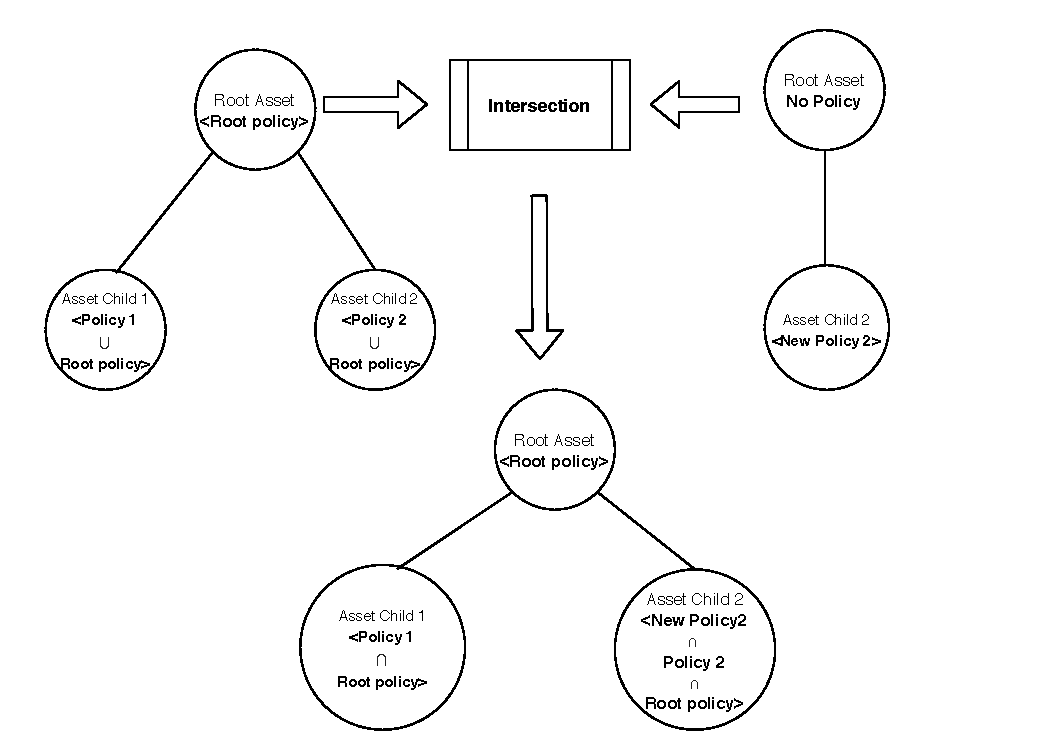
\includegraphics[scale=.60]{../immagini/wrongProp.pdf}
\caption{Intersezione di policy precedentemente in ambiente collaborativo}
\label{wrongProp}
\end{figure}
Sull'\textit{Asset Child 2} si ha l'effetto desiderato: la risorsa non è più considerata in ambiente collaborativo ed ha come regole quelle ottenute dall'intersezione delle policy che la riguardano. Per quanto concerne la policy finale di \textit{Asset Child 1} si ha che nonostante l'unica policy introdotta sia \textit{New Policy 2} la propagazione dell'ambiente non collaborativo produce effetti anche su \textit{Policy 1}.\\
La problematica appena presentata è stata trattata aggiungendo i seguenti passi all'algoritmo mostrato fino ad ora:
\begin{enumerate}
\item recupero degli asset che hanno subito una modifica di policy, ovvero le risorse che hanno in entrambe le policy almeno una regola che le riguarda. Questi nodi sono un sottoinsieme dei nodi comuni alle policy.
\item recupero dell'intero sottografo che ha come origine un nodo modificato;
\item reset della policy originaria per i nodi recuperati nei passi precedenti, senza attuare propagazioni.
\end{enumerate}
Il sottoagrafo così recuperato è l'insieme degli asset effettivamente interessati da un'operazione di intersezione o unione. Questa affermazione può essere dimostrata come segue:
\begin{enumerate}
\item sia C l'insieme degli asset regolati da entrambe le policy;
\item sia M un sottoinsieme di C formato dai nodi per cui entrambe le policy presentano almeno una regola;
\item sia F l'insieme dato dall'unione dei nodi appartenti ai sottografi di tutti i nodi in M;
\item sia R l'unione di M ed F;
\item gli elementi di R sono i nodi nel sottografo interessato dall'operazione di intersezione o unione delle policy;
\item supponendo per assurdo che altri nodi siano parte del sottografo:
\begin{enumerate}
\item un nodo non appartenente a C è, per definizione, interessato in modo diretto solamente da una policy; si noti che F può contenere nodi non appartenenti a C;
\item un nodo non appartenente ad M con una sola policy definita non subisce modifiche alla sua policy, di conseguenza la propagazione della sua policy finale ai nodi figli è già stata attuata;
\item un nodo non appartenente ad M con entrambe le policy non definite non dà alcun contributo alla propagazione; inoltre non avendo alcuna policy, anche tutti i suoi nodi parent non hanno policy definite;
\item se un nodo non appartiene ad F, nessuno dei nodi parent appartiene ad F o M, di conseguenza ha già subito eventuali propagazioni di policy ed ha già propagato le proprie regole.
\end{enumerate}
Queste modifiche producono i seguenti effetti:
\begin{figure}[H]
\centering
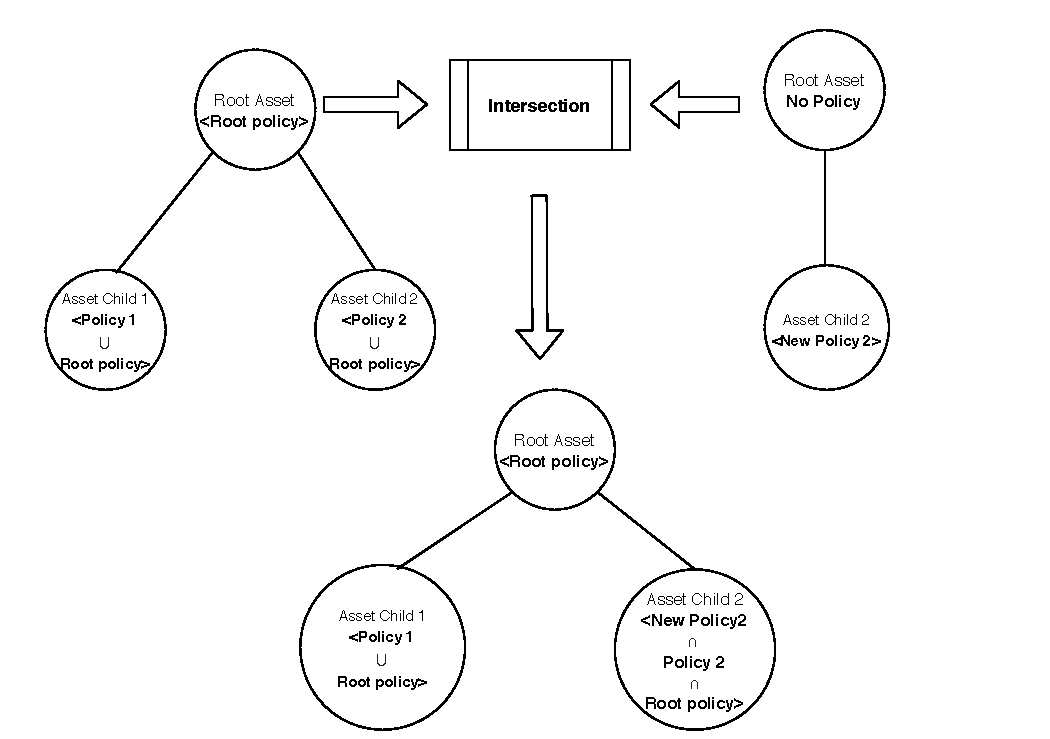
\includegraphics[scale=0.6]{../immagini/correctProp.pdf}
\caption{Intersezione di policy precedentemente in ambiente collaborativo senza override di ambiente}
\label{correctProp}
\end{figure}
\end{enumerate}
\section{Produzione policy ODRL}\label{produceSection}
Il produttore di documenti ODRL è l'ultimo componente della pipeline per il policy merging. Il ruolo svolto risulta essere di comunicazione tra i wrapper prodotti dalla logica di merging ed il modulo I/O del framework Jena. Le funzionalità sono attuate mediante la seguente procedura:
\begin{enumerate}
\item tramite le \textit{Core RDF API} fornite da Jena si crea un nuovo modello RDF;
\item tramite il gestore gerarchia asset della policy finale si recupera una mappa che collega l'URI di un asset alla propria policy;
\item per ogni URI:
\begin{enumerate}
\item si aggiunge al modello una risorsa relativa all'asset;
\item si recuperano le risorse relative ai parent degli asset;
\item a tutte le risorse recuperate al passo precedente si aggiunge alla proprietà \textit{odrl:partOf} il nuovo nodo;
\item per ogni regola nella policy si crea un nodo;
\item i nodi relativi alle regole vengono inseriti nella proprietà \textit{permission} o \textit{prohibition} del nuovo nodo relativo all'asset;
\end{enumerate}
\item viene settato il namespace relativo al contesto ODRL;
\item il modello viene utilizzato dal modulo I/O che ne produce la corrispondente serializzazione Turtle.
\end{enumerate}
Il documento RDF finale prodotto ha le seguenti proprietà:
\begin{itemize}
\item ogni regola espressa appare una sola volta per target;
\item ogni asset ha una propria definizione;
\item la lista mostrata nelle proprietà \textit{partOf} non contiene ripetizioni.
\end{itemize}
\chapter{Valutazione dei risultati}
I principali obiettivi che questo lavoro di tesi si è posto sono stati esposti nella sezione \ref{problematiche} e riguardano due aree principali:
\begin{enumerate}
\item l'assenza da parte di ODRL di un metodo per trattare policy conflittuali all'interno dei casi d'uso individuati da MOSAICrOWN;
\item controllo ineficciente di una regola, poiché con query puntuali sul documento ODRL è possibile ottenere informazioni non corrette sulla regolamentazione di un'azione. Attualmente risulta necessario controllare l'intero file per avere certezze su quanto è permesso su di un asset.
\end{enumerate}
Il tool sviluppato affronta e risolve entrambe queste problematiche nel caso di azioni prive di \textbf{constraint}. La soluzione proposta non è applicabile solamente ai casi d'uso di MOSAICrOWN, come quelli relativi a mercati digitali dove gli asset possono avere più possessori, ma anche a scenari più tradizionali, come la definizione di policy d'accesso a risorse in un sistema operativo.\\
Per risolvere la prima problematica il focus principale è stato lo sviluppo di procedure che supportassero le operazioni di merging \textbf{unione} ed \textbf{intersezione}. Tali operazioni identificano i principali ambienti dove è possibile definire policy d'accesso: \textbf{collaborativo} e \textbf{non collaborativo}.\\
La seconda problematica è stata affrontata su più livelli:
\begin{itemize}
\item a livello di \textbf{singola} policy: durante la lettura di un documento ODRL che definisce una policy d'accesso il framework si occupa di inferire quelli che sono le \textbf{implicazioni} tra le regole seguendo le definizioni date dall' \textit{ODRL Common Vocabulary}. In questo modo si impediscono ambiguità su regole interne alla policy dove una sottoazione è permessa ma non l'azione padre è invece vietata;
\item a livello di \textbf{asset}: durante la lettura del documento di ODRL il framework si occupa di inferire in base all'ambiente specificato per la policy le regole che un asset eredita dai propri parent. Ottenute queste regole si attua la procedura vista per policy singola.
\end{itemize}
Entrambi i procedimenti appena esposti vengono attuati dall'architettura osservabile in figura \ref{procMergin} i cui componenti sono stati esposti in dettaglio all'interno del capitolo \ref{implementazioniCh} relativo all'implementazione della soluzione. L'output della pipeline è un nuovo documento di policy ODRL che rappresenta il risultato dell'operazione desiderata.\\
Si può notare come la soluzione sia modulare: non si è costretti ad utilizzare il tool unicamente per procedure di merging, poiché risulta possibile sfruttare ogni componente, e relativi sottocomponenti, senza l'ausilio degli altri. Questo permette sia lo sfruttamento delle singole funzionalità di ogni porzione del lavoro sia la possibilità di estensione o sostituzione di un componente.\\
\section{Esempi di casi d'uso}
All'interno di questa sezione vengono mostrati casi d'uso dalla complessità crescente supportati dal lavoro di tesi. I risultati ottenuti effettuando query sull'output del policy merging vengono confrontati con ciò che è possibile effettuare solamente sui documenti ODRL originali.
\subsection{Merging di policy relative ad un singolo asset}
Casistica più semplice in assoluto. Risulta utile per comprendere il comportamento del tool e cosa si intende con procedura di merging. Di seguito i file ODRL utilizzati come input:
\begin{lstlisting}[language=json,firstnumber=1,caption={Policy ODRL su singolo asset},captionpos=b,label=mergingOnSingle1]
{  "uid":"http://singleExample1",
   "type":"Policy",
   "@context":"http://www.w3.org/ns/odrl.jsonld",
   "permission":[
      {
         "target":"http://Child2",
         "action":"display"
      },
      {
         "target":"http://Child2",
         "action":"stream"
      }
   ],
   
   
   "prohibition":[
      {
         "target":"http://Child2",
         "action":"uninstall"
      }
   ]
}
\end{lstlisting}
\begin{lstlisting}[language=json,firstnumber=1,caption={Policy ODRL su singolo asset},captionpos=b,label=mergingOnSingle2]
{
   "uid":"http://singleExample2",
   "type":"Policy",
   "@context":"http://www.w3.org/ns/odrl.jsonld",
   "permission":[

      {
         "target":"http://Child2",
         "action":"play"
      },
      {
         "target":"http://Child2",
         "action":"install"
      }
      ,
            {
               "target":"http://Child2",
               "action":"uninstall"
            }
   ],
   "prohibition":[
      {
         "target":"http://Child2",
         "action":"delete"
      }
   ]
}
\end{lstlisting}
Di seguito, invece, vi sono i file prodotti, 1 per possibile operazione:
\begin{lstlisting}[language=json,firstnumber=1,caption={Risultato dell'intersezione delle policy nei listing \ref{mergingOnSingle1} e \ref{mergingOnSingle2}},captionpos=b,label=intersectionSingle]
@prefix odrl:  <http://www.w3.org/ns/odrl/2/> .

<http://single>  a odrl:Set ;
 odrl:permission   ( [ a odrl:Permission ;
                       odrl:action  odrl:display ;
                       odrl:target  <http://Child2>
                     ]
                    ) ;
odrl:prohibition  ( [ a odrl:Prohibition ;
                      odrl:action  odrl:uninstall ;
                      odrl:target  <http://Child2>
                     ]
                     [ a odrl:Prohibition ;
                       odrl:action  odrl:delete ;
                       odrl:target  <http://Child2>
                       ]
                    ) .

<http://Child2>  odrl:partOf  <EveryAsset> .
\end{lstlisting}
\newpage
\begin{lstlisting}[language=json,firstnumber=1,caption={Risultato dell'unione delle policy nei listing \ref{mergingOnSingle1} e \ref{mergingOnSingle2}},captionpos=b,label=unionSingle]
@prefix odrl:  <http://www.w3.org/ns/odrl/2/> .
<http://singleUnion>  a odrl:Set ;
odrl:permission   ( [ a odrl:Permission ;
                      odrl:action  odrl:play ;
                      odrl:target  <http://Child2>
                     ]
                     [ a odrl:Permission ;
                     odrl:action  odrl:display ;
                     odrl:target  <http://Child2>
                     ]
                     [ a            odrl:Permission ;
                     odrl:action  odrl:install ;
                     odrl:target  <http://Child2>
                     ]
                     [ a odrl:Permission ;
                       odrl:action  odrl:stream ;
                       odrl:target  <http://Child2>
                     ]
                  ) ;
odrl:prohibition  ( [ a odrl:Prohibition ;
                     odrl:action  odrl:uninstall ;
                     odrl:target  <http://Child2>
                     ]
                     [ a odrl:Prohibition ;
                     odrl:action  odrl:delete ;
                     odrl:target  <http://Child2>
                     ]
                     ) .

<http://Child2>  odrl:partOf  <EveryAsset> .

\end{lstlisting}
Il risultato è riassunto dalla seguente immagine:
\begin{figure}[H]
\centering
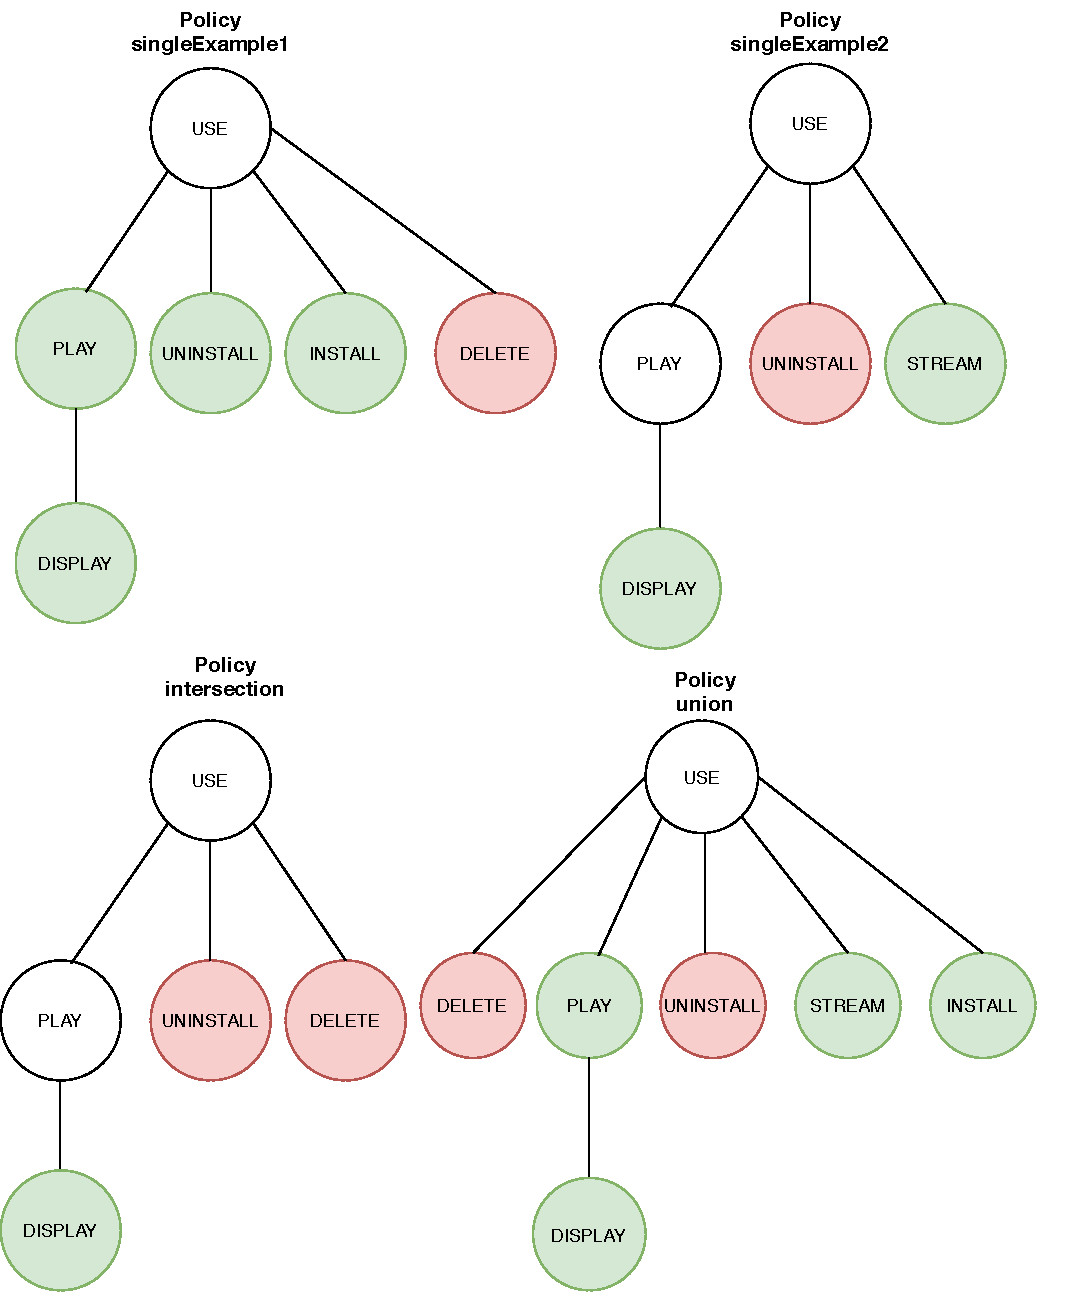
\includegraphics[scale=.50]{../immagini/singlePolicyExample.pdf}
\caption{Albero delle regole delle varie policy all'interno dell'esempio}
\label{singleResult}
\end{figure}
Vantaggi osservabili utilizzando i file mostrati nei listing \ref{unionSingle} e \ref{intersectionSingle}:
\begin{itemize}
\item risulta possibile ottenere la regolamentazione di un'azione mediante una query puntuale accedendo ad un singolo file. L'implementazione baseline è invece costretta ad accedere ad almeno 2 file;
\item l'implementazione baseline è anche costretta a controllare l'intera gerarchia dell'azione per cui si esegue il check, effettuando un ulteriore accesso al vocabolario ODRL;
\item la procedura di merging può essere considerata computazionalmente più onerosa rispetto a quella baseline, poiché aggiunge overhead relativi alla gestione della gerarchia degli asset, inutilizzati in questo caso;
\item l'overhead aggiunto al punto precedente è però da considerarsi un costo pagato una singola volta, a discapito invece dell'approccio baseline che deve ogni volta ricercare le informazioni relative alle \textit{action}.
\end{itemize}
Il vantaggio principale dell'approccio adottato all'interno della tesi risiede nell'aver prodotto un documento non ambiguo e concentrato delle informazioni relative alle policy d'accesso. Tale costo è pagato solo all'inserimento di un nuovo documento ODRL, ottenendo una procedura più efficiente nel lungo termine.

\subsection{Merging di policy relative ad asset con gerarchia ad albero}
Questa casistica risulta la seconda meno complessa: le 2 policy lavorano sugli stessi asset, i quali hanno una struttura gerarchica ad albero, ovvero ogni nodo ha un solo padre possibile. Nella trattazione di questo caso d'uso viene dato per scontato il corretto funzionamento di intersezione tra singole policy, focalizzandosi invece su quello che è il comportamento del tool nel propagare le policy.\\
La casistica più interessante da studiare risulta essere l'\textit{intersezione} di ambienti \textit{non collaborativi}.
\begin{table}[H]
\begin{tabular}{|c|c|c|c|c|c|c|}
\hline
{} & \makecell{\textbf{Root} \\\textbf{Policy 1}} & \makecell{\textbf{Root} \\\textbf{Policy 2}} & \makecell{\textbf{Child 1} \\\textbf{Policy 1}} & \makecell{\textbf{Child 1} \\\textbf{Policy 2}} & \makecell{\textbf{Child 2} \\\textbf{Policy 1}} & \makecell{\textbf{Child 2} \\\textbf{Policy 2}} \\
\hline
{play} & \cellcolor{green!25} & \cellcolor{green!25} & {} & {} & {} & {} \\
\hline
{diplay} & \cellcolor{green!25}& \cellcolor{green!25} & {} & \cellcolor{green!25} & {} & {} \\
\hline
{install} & \cellcolor{green!25} & \cellcolor{green!25} & \cellcolor{green!25} & \cellcolor{green!25} & {} &\cellcolor{green!25} \\
\hline
{annotate} & \cellcolor{green!25} & {} & {} & {} & \cellcolor{green!25} & \cellcolor{red!25} \\
\hline
{delete} & \cellcolor{red!25} & \cellcolor{red!25} & {}&  {} & \cellcolor{red!25} & {}\\
\hline
{stream} & {} & {} & \cellcolor{red!25} & \cellcolor{red!25} & {} &  {}\\
\hline

\end{tabular}
\caption{Regolamentazione delle policy prima dell'applicazione di ambiente non collaborativo e intersezione}
\label{tableTree}
\end{table}
La struttura della gerarchia dello scenario è visibile in figura \ref{treeExampleImg}. In caso di ambiente \textbf{non collaborativo} si attua un'intersezione tra la policy del nodo padre ed i suoi figli. L'operazione d'intersezione finale interseca le varie policy ad ogni livello, per poi andare ad attuare la propagazione di ambiente \textbf{non collaborativo} sull'intero albero. Il risultato finale in questo caso è quanto segue:

\begin{table}[H]
\centering
\begin{tabular}{|c|c|c|c|}
\hline
{} & \makecell{\textbf{Root}} & \makecell{\textbf{Child 1}} & \makecell{\textbf{Child 2}} \\
\hline
{play} & \cellcolor{green!25} & {}& {} \\
\hline
{diplay} & \cellcolor{green!25}& {} & {} \\
\hline
{install} & \cellcolor{green!25} & \cellcolor{green!25} & {}\\
\hline
{annotate} & {} & {} & \cellcolor{red!25} \\
\hline
{delete} & \cellcolor{red!25} & \cellcolor{red!25} & \cellcolor{red!25} \\
\hline
{stream} & {} & \cellcolor{red!25} & {}\\
\hline

\end{tabular}
\caption{Regole all'interno della policy prodotta in output}
\label{tableTreeFinal}
\end{table}
Dalla tabella \ref{tableTreeFinal} si nota che:
\begin{itemize}
\item una policy sulla root mantiene i suoi permessi solo se presenti in entrambe le policy intersecate, per effetto dell'operazione di \textbf{intersezione};
\item una policy su un nodo figlio mantiene i suoi permessi se presenti in entrambe le policy intersecate e se anche la policy finale del nodo padre presenta tali permessi, quest'ultimo effetto è dato dall'ambiente \textbf{non collaborativo}.
\end{itemize}
Questa casistica risulta la maggiormente interessante poiché:
\begin{itemize}
\item l'intersezione di ambienti collaborativi in questa situazione produce come risultato la propagazione della policy della radice a tutti i nodi. Questo è causato dall'operazione di unione preliminare poi seguita da quella di intersezione;
\item i casi relativi all'unione di policy sono poco interessanti, poiché non avviene alcun filtraggio particolare delle regole.
\end{itemize}
Un'ulteriore motivazione d'interesse verso questa casistica è il fatto che può essere considerata una prima modellizzazione degli scenari d'interesse di MOSAICrOWN: un eventuale utente che possiede l'\textit{asset child 1}, qualora volesse modificare la propria policy d'accesso, scatenerebbe questa casistica(salvo la propagazione dell'intersezione verso gli altri asset).\\
In questo caso il tool sviluppato porta i medesimi vantaggi già mostrati nel caso precedente, aggiungendo i seguenti:
\begin{itemize}
\item in questo caso risulta necessaria un'ulteriore query da parte della baseline per recuperare la gerarchia relativa all'asset interessato dall'accesso;
\item a seconda della tipologia di nodo, risulterà quindi necessario recuperare anche lo stato dell'azione all'interno della gerarchia dell'asset, tenendo conto del fatto che non è stata attuato alcun tipo di propagazione nei documenti originali;
\item il costo dell'esecuzione dell'approccio baseline in questo caso si avvicina molto a quello che si ha per attuare il merging di policy, rendendo evidente il vantaggio portato dalla produzione di una policy output;
\item l'approccio implementato permetterebbe ad un owner degli asset di valutare la perdita di valore introdotta da una modifica alla propria policy d'accesso.
\end{itemize}
\begin{figure}[H]
\centering
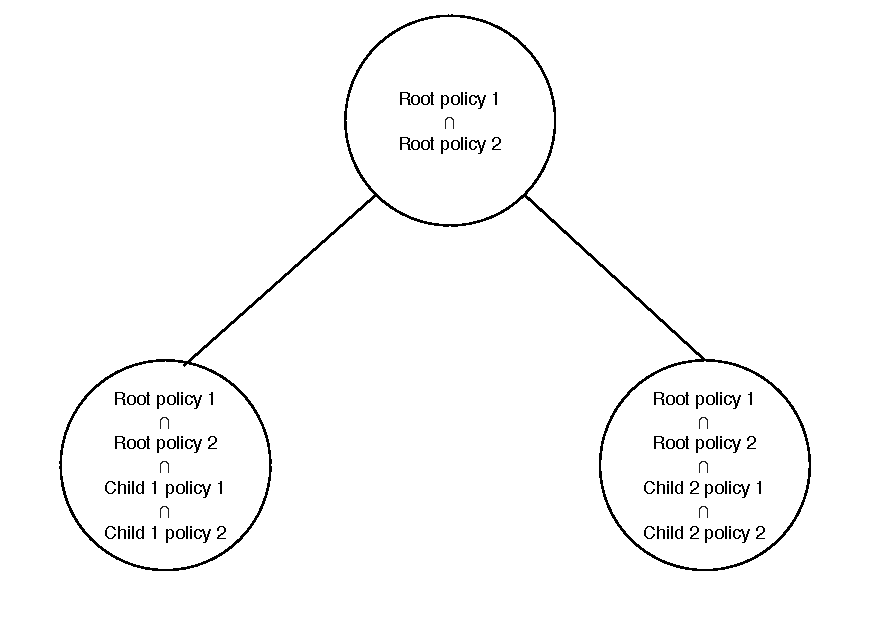
\includegraphics[scale=.50]{../immagini/treePolicyExample.pdf}
\caption{Policy finali del caso d'uso}
\label{treeExampleImg}
\end{figure}
\subsection{Merging di policy relative a gerarchie differenti}
In questo scenario, le 2 policy operano su gerarchie parzialmente sovrapposte. La casistica trattata sarà in questo caso l'\textit{intersezione} di ambienti \textit{collaborativi}. La procedura seguita dall'algoritmo è riassunta nella seguente figura:
\begin{figure}[H]
\centering
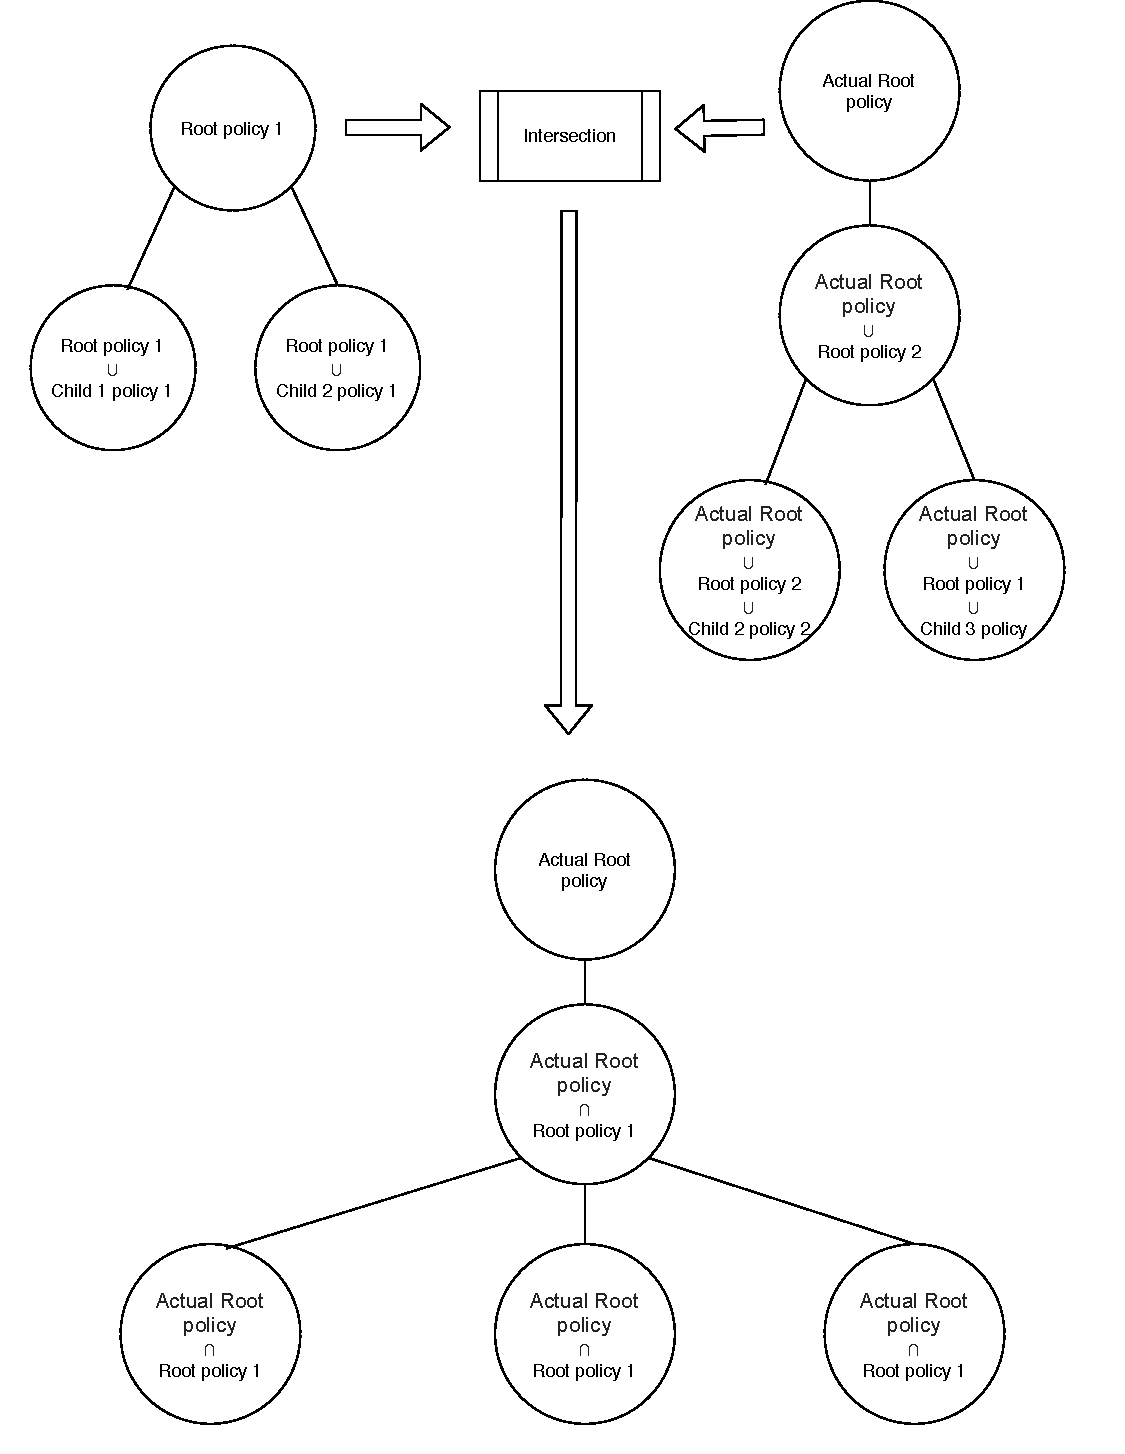
\includegraphics[scale=.5]{../immagini/treeNewNodesExample.pdf}
\caption{Procedura seguita per l'intersezione di 2 policy in ambiente collaborativo con l'aggiunta di nuovi nodi padre e foglia}
\label{treeNewNodeExample}
\end{figure}
Questa casistica assume maggiore interesse rispetto allo scenario precedente, poiché l'aggiunta di nuovi parent all'interno della gerarchia modifica quello che è il comportamento dell'unione seguita da intersezione: nel caso precedente questo portava alla replica dell'intersezione dei nodi negli altri nodi; in questo caso le differenze nella gerarchia fanno in modo che cambi il punto dal quale inizia la replica. Si noti che le operazioni a cui fa riferimento la figura \ref{treeNewNodeExample} sono relative ai permessi delle policy, che vengono ``mascherati'' dalla sequenza unione-intersezione. Eventuali i divieti delle policy non visibili in figura sono comunque propagati lungo l'albero.\\
I vantaggi introdotti in questo caso sono analoghi a quelli dello scenario precedente, poiché si tratta semplicemente di un'estensione a livello logico delle stesse casistiche. 
\subsection{Merging di policy relative ad asset con gerarchia complessa}
Quest'ultimo scenario mostrato risulta essere il più complesso dal punto di vista della gerarchia degli asset rappresentata da un DAG anziché da un albero. L'esempio è caratterizzato dalle seguenti proprietà:
\begin{itemize}
\item ambienti iniziali collaborativi;
\item intersezione di policy;
\item aggiunta di parent da parte di una policy;
\item aggiunta di una nuova foglia da parte di una policy;
\item valutazione dei risultati utilizzando sia l'algoritmo senza e con l'estensione introdotta nella sezione \ref{estensioneAlg}.
\end{itemize}
La struttura precedente al merging è visibile nella figura sottostante:
\begin{figure}[H]
\centering
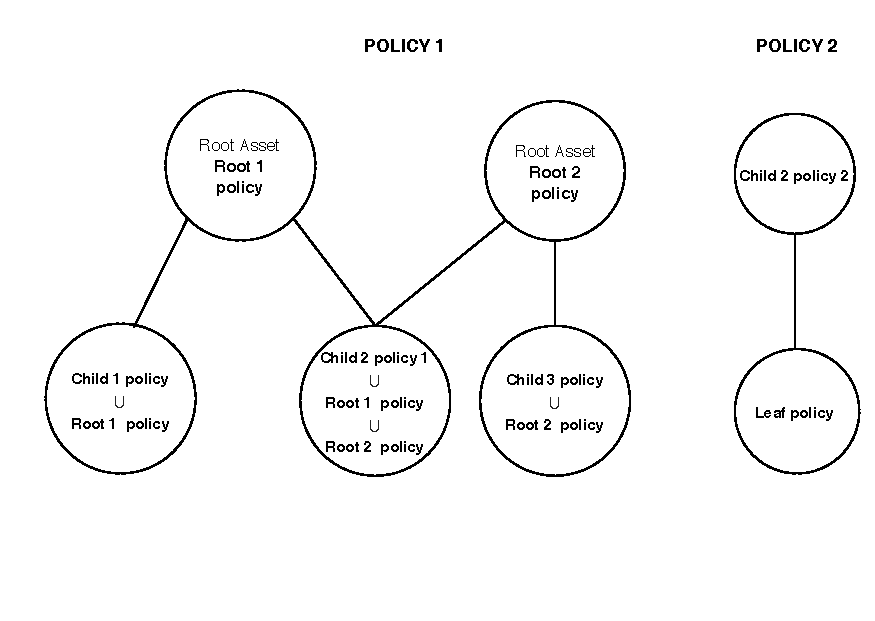
\includegraphics[scale=.65]{../immagini/DAGExample.pdf}
\caption{Struttura dei DAG regolati dalle policy}
\label{DAGStructureExample}
\end{figure}
All'interno della tabella \ref{tableInitialDAG} sono presenti i permessi utilizzati come esempio. Le regole sono da intendersi come input allo strumento e quindi precedenti all'applicazione dell'ambiente collaborativo.  Le tabelle \ref{finalDAGProp} e \ref{finalDAGNoProp} contengono invece i permessi nella policy prodotta a seconda del metodo di propagazione scelto.
\begin{table}[h]
\begin{tabular}{|c|c|c|c|c|c|c|c|}
\hline
{} & \makecell{\textbf{Root 1}} & \makecell{\textbf{Root 2}} & \makecell{\textbf{Child 1}} & \makecell{\textbf{Child 2} \\\textbf{Policy 1}} & \makecell{\textbf{Child 2} \\\textbf{Policy 2}} & \makecell{\textbf{Child 3}} & \makecell{\textbf{Leaf}}\\
\hline
{play} & \cellcolor{green!25} & \cellcolor{green!25} & {} & {} & {} & {}& {}  \\
\hline
{diplay} & \cellcolor{green!25}& \cellcolor{green!25} & {} & {} & \cellcolor{green!25} & {} & \cellcolor{green!25} \\
\hline
{install} & \cellcolor{green!25} & {} & {}& {} & {} &{} & {} \\
\hline
{annotate} & {}& {} & \cellcolor{green!25}  & {} & {}& {} & {} \\
\hline
{delete} & \cellcolor{green!25} & {} & {}&  {} & {} & {}& \cellcolor{green!25} \\
\hline
{stream} & {} & \cellcolor{green!25} & {} & {} & {} &  {}& {} \\
\hline
{anonymize} & {} & {} & {} & \cellcolor{green!25} & \cellcolor{green!25} &  {}& {} \\
\hline
{translate} & {} & {} & {} & {} & {} &  \cellcolor{green!25}& {} \\
\hline

\end{tabular}
\caption{Permessi espresi esplicitamente dalle 2 policy di cui si fa l'intersezione}
\label{tableInitialDAG}
\end{table}
\begin{table}[H]
\begin{tabular}{|c|c|c|c|c|c|c|}
\hline
{} & \makecell{\textbf{Root 1}} & \makecell{\textbf{Root 2}} & \makecell{\textbf{Child 1}} & \makecell{\textbf{Child 2} }  & \makecell{\textbf{Child 3}} & \makecell{\textbf{Leaf}}\\
\hline
{play} & \cellcolor{green!25} & \cellcolor{green!25} & \cellcolor{green!25} & {}& \cellcolor{green!25}& {}  \\
\hline
{diplay} & \cellcolor{green!25}& \cellcolor{green!25} & \cellcolor{green!25} & \cellcolor{green!25} & \cellcolor{green!25} & \cellcolor{green!25} \\
\hline
{install} & \cellcolor{green!25} & {} & \cellcolor{green!25}& {} &{} & {} \\
\hline
{annotate} & {}& {} & {}  & {} &  {} & {} \\
\hline
{delete} & \cellcolor{green!25} & {} & \cellcolor{green!25}&  {} & {}& {} \\
\hline
{stream} & {} & \cellcolor{green!25} & {} & {}&   \cellcolor{green!25}& {} \\
\hline
{anonymize} & {} & {} & {} & {} &  {}& {} \\
\hline
{translate} & {} & {} & {} & {}  &  {}& {} \\
\hline

\end{tabular}
\caption{Permessi in seguito all'intersezione con propagazione dell'ambiente sull'intero DAG}
\label{finalDAGProp}
\end{table}
\begin{table}[h]
\begin{tabular}{|c|c|c|c|c|c|c|}
\hline
{} & \makecell{\textbf{Root 1}} & \makecell{\textbf{Root 2}} & \makecell{\textbf{Child 1}} & \makecell{\textbf{Child 2} }  & \makecell{\textbf{Child 3}} & \makecell{\textbf{Leaf}}\\
\hline
{play} & \cellcolor{green!25} & \cellcolor{green!25} & \cellcolor{green!25} & {}& \cellcolor{green!25}& {}  \\
\hline
{diplay} & \cellcolor{green!25}& \cellcolor{green!25} & \cellcolor{green!25} & \cellcolor{green!25} & \cellcolor{green!25} & \cellcolor{green!25} \\
\hline
{install} & \cellcolor{green!25} & {} & \cellcolor{green!25}& {} &{} & {} \\
\hline
{annotate} & {}& {} & \cellcolor{green!25}  & {} &  {} & {} \\
\hline
{delete} & \cellcolor{green!25} & {} & \cellcolor{green!25}&  {} & {}& {} \\
\hline
{stream} & {} & \cellcolor{green!25} & {} & {}&   \cellcolor{green!25}& {} \\
\hline
{anonymize} & {} & {} & {} & {} &  {}& {} \\
\hline
{translate} & {} & {} & {} & {}  &  \cellcolor{green!25}& {} \\
\hline

\end{tabular}
\caption{Permessi in seguito all'intersezione con propagazione solo su asset interessati dal merging}
\label{finalDAGNoProp}
\end{table}
Come risulta possibile notare dalla tabella \ref{finalDAGProp} forzare l'ambiente in base all'operazione di merging effettuata può portare ad effetti indesiderati su porzioni del DAG non interessate dalla procedura:
\begin{itemize}
\item l'asset \textit{Child 1} perde il permesso relativo all'azione \textit{annotate};
\item l'asset \textit{Child 3} perde il permesso relativo all'azione \textit{translate}.
\end{itemize}
All'interno dello strumento viene comunque lasciata questa possibilità poiché questo caso d'uso può avere comunque delle applicazioni.\\
La tabella \ref{finalDAGNoProp} mostra invece quello che è l'effetto desiderato nella maggior parte dei casi applicativi:
\begin{itemize}
\item solamente l'asset \textit{Child 2} perde le i permessi che potrebbe mantenere in ambiente collaborativo, ovvero \textit{anonymize};
\item le risorse restanti mantengono le policy in ambiente collaborativo;
\item i nodo figlio di \textit{Child 2}, pur non essendo interessato direttamente dall'operazione di intersezione, risulta in ambiente non collaborativo.
\end{itemize}
La procedura per ottenere gli effetti esposti nelle tabelle \ref{finalDAGProp} e \ref{finalDAGNoProp} sono riassunti nella figura \ref{DAGResult}. 

Lo scenario mostrato risulta interessante poiché è possibile notare quali siano gli effetti dati dalla più ampia variaretà di casistiche possibile. Lo strumento risulta in grado di trattare queste casistiche, dando una base per l'interrogazione efficiente anche con relazioni complesse tra gli asset. \\
Quest'ultimo caso d'uso non è però l'effettiva casistica presa in esame da MOSAICrOWN, la cui caratterizzazione sarebbe la seguente:
\begin{itemize}
\item ambienti iniziali non collaborativi, avendo collezioni multi owner;
\item intersezione di policy, avendo collezioni multi owner;
\item aggiunta di un parent rappresentante la collezione di cui si fa parte nel mercato digitale;
\item aggiunta o modifica di una foglia rappresentante la collezione dati dell'owner che vuole aggiungersi al mercato;
\item risulta necessario l'utilizzo della procedura di merging estesa.
\end{itemize}
Questa casistica risulta però più limitata da un punto di vista della presentazione dei risultati raggiunti: non vi è un cambiamento di ambiente e la gerarchia può essere espressa mediante un albero. Infine per MOSAICrOWN risulta interessante solamente l'utilizzo dell'algoritmo esteso: cambiamenti portati da un owner non devo avere effetti su dati sui quali non può definire regole.
\begin{figure}[H]
\centering
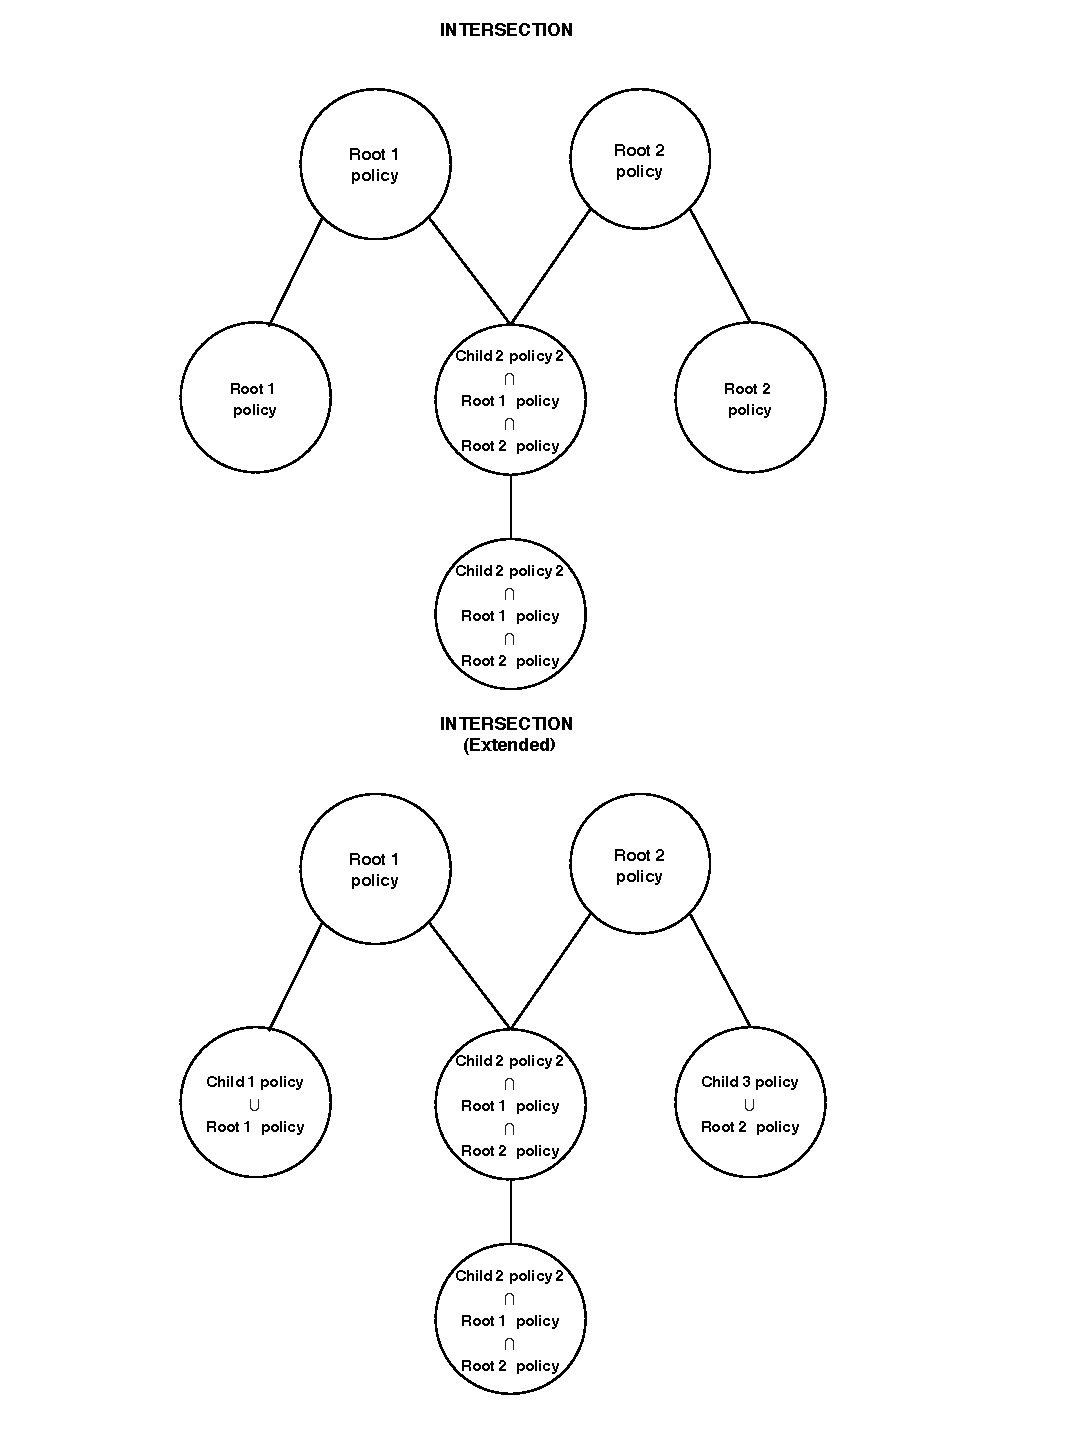
\includegraphics[scale=.80]{../immagini/DAGExampleRES.pdf}
\caption{}
\label{DAGResult}
\end{figure}
\section{Possibili sviluppi futuri}
In questa sezione si discutono quelli che possono essere gli sviluppi futuri del lavoro svolto. In particolare si trattano i seguenti aspetti:
\begin{itemize}
\item effettivo sistema per il deployment del tool;
\item supporto alle gestione della cronologia delle operazioni;
\item supporto ad azioni con \textbf{constraint}.
\end{itemize}
I primi due temi non sono stati approfonditi durante la stesura della tesi poiché non direttamente inerenti al merging di policy. L'ultimo tema, invece, non è stato trattato poiché la generalizzazione dei vincoli relativi ad un'azione dipende dai vari domini possibili. 
\paragraph{Possibile deployment del tool}\mbox{}\\
Per sfruttare completamente i vantaggi portati dalla procedura sviluppata risulta necessario effettuare il merging di policy solo all'inserimento di un documento ODRL all'interno del mercato digitale. Tra le possibili serializzazioni RDF vi è il formato JSON-LD. Questo formato può essere sfruttato all'interno di basi di dati NoSQL come ad esempio MongoDB.\\
Per quanto concerne l'effettivo inserimento di un documento ODRL all'interno della base di dati del mercato digitale si potrebbe esporre un REST Service dove il corpo delle richieste è un documento JSON avente i seguenti campi:
\begin{itemize}
\item operazione di merging che si desidera effettuare;
\item oggetto JSON contenente la serializzazione JSON-LD di una policy;
\item identificativo della collezione al quale si vuole prendere parte.
\end{itemize}
In questo modo il sistema avrebbe tutte le informazioni necessarie per attuare il merging tra la policy attuale delle collezione esposta nel mercato digitale e quella inviata al servizio REST.
\paragraph{Possibile gestione della cronologia delle operazioni}\mbox{}\\
All'interno del mercato digitale risulta possibile che i vari owner non vogliano solamente aggiungere dati ad una collezione ma modificarne la policy o rimuovere i propri dati dal mercato. Per supportare questo tipo di operazioni è necessaria la rappresentazione della cronologia delle operazioni che hanno portato una policy al suo stato attuale.\\
La rappresentazione che viene proposta è riassunta nella seguente immagine:
\begin{figure}[H]
\centering
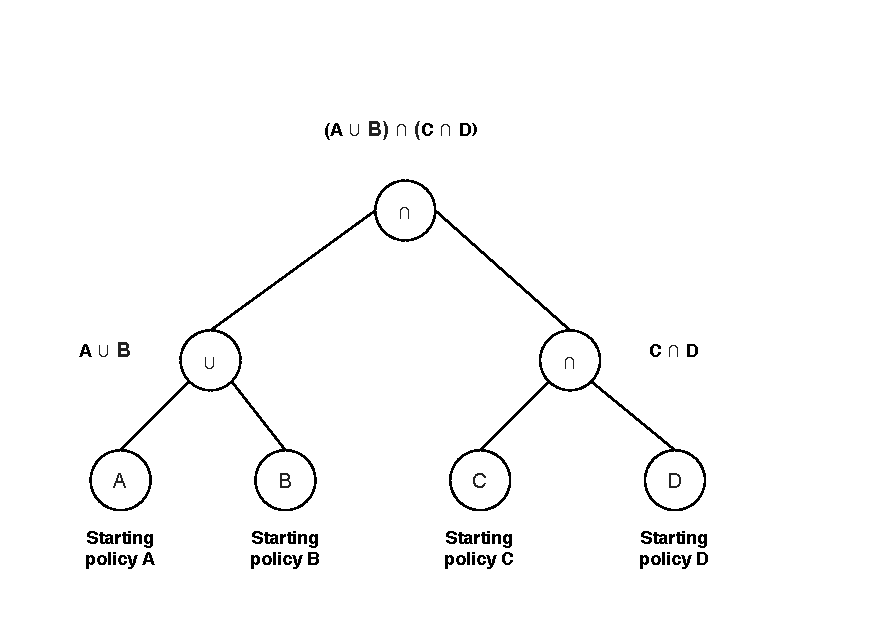
\includegraphics[scale=.50]{../immagini/historyFirst.pdf}
\caption{Esempio di rappresentazione della cronologia di operazioni che portano allo stato finale di una policy}
\label{historyFirst}
\end{figure}
Questa rappresentazione può essere attuata seguendo due metodi:
\begin{itemize}
\item arricchendo la sintassi ODRL inserendo termini relativi al processo di merging. In questo modo si seguono i princici dei \textit{Linked Data} poiché da una policy è possibile raggiungere i vari documenti che hanno contribuito alla sua creazione;
\item inserendo in una base di dati record relativi alle operazioni intraprese su una policy. Questo approccio risulta attuabile anche in database relazionali ma è meno vicino ai principi di sviluppo di ODRL.
\end{itemize}
In ognuno dei due casi se una delle policy originali venisse rimossa o modificata l'unica operazione necessaria per aggiornare i documenti finali sarebbe ripercorrere l'albero delle operazioni. Prendendo ad esempio la figura \ref{historyFirst}: se si volesse rimuovere la policy B si seguirebbe il procedimento riassunto nella seguente figura:
\begin{figure}[H]
\centering
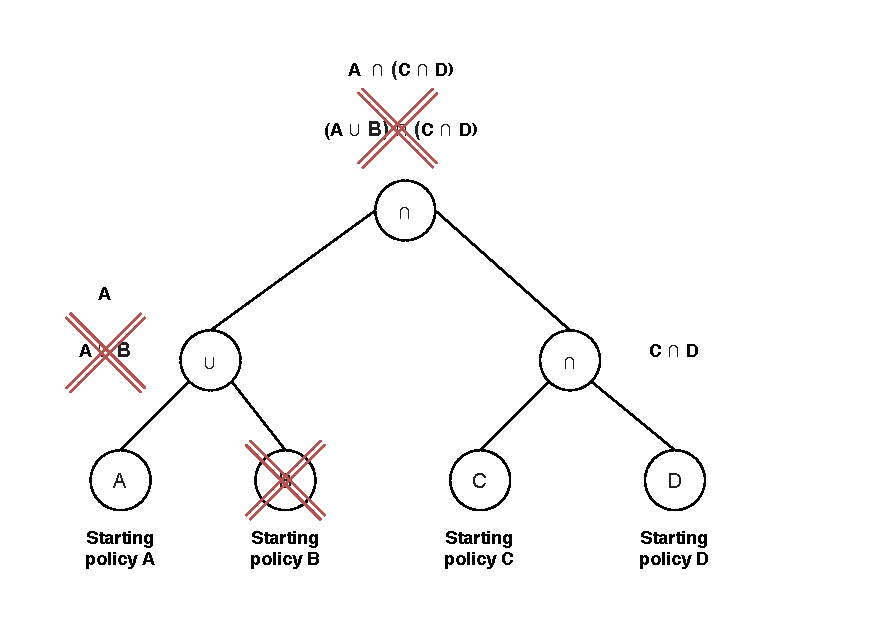
\includegraphics[scale=.50]{../immagini/historySecond.pdf}
\caption{Rappresentazione della procedura attuata in seguito alla rimozione della policy B}
\label{historySecond}
\end{figure}
\paragraph{Trattazione regole con constraint}\mbox{}\\
Come mostrato all'interno della sezione \ref{ConstraintODRL}, ODRL permette la definizione di \textbf{refinement} sulle azioni regolate da una policy. Questo aspetto non è stato trattato all'interno del lavoro di tesi per le seguenti motivazioni:
\begin{itemize}
\item i dati contenuti in queste proprietà possono essere poco strutturati. Si prenda come esempio il listing \ref{esempioRef} dove la proprietà \textit{unit} è definibile attraverso un link che spiega quale sia l'unità di misura utilizzata. Questo comporta la definizione di procedure specifiche rispetto al dominio e quindi poco generalizzabili;
\item come visibile all'interno dell'\textit{ODRL Information Model}\cite{ODRLinfMod} la struttura relativa ai \textit{Constraint} è soggetta a cambiamenti; per esempio risultano tra i pochi punti di non compatibilità con le vecchie versioni di ODRL. Per ottenere uno strumento il più stabile possibile si è preferito non lavorare su questa porzione del linguaggio che risulta in fase di definizione. 
\end{itemize}
Alla luce di queste problematiche per riuscire ad utilizzare questi costrutti all'interno di un mercato digitale risulta necessario discretizzare il \textit{range} utilizzabile in queste proprietà. Questo procedimento andrebbe a ridurre la flessibilità del linguaggio ma, allo stesso tempo, permetterebbe di attuare logiche di merging anche su questa porzione di ODRL.  
\chapter{Conclusione}
La soluzione implementata risolve le problematiche individuate in ODRL in molteplici scenari, compresi quelli individuati in MOSAICrOWN. Tali problemi riguardavano l'assenza di politiche per risolvere conflitti tra policy in un contesto multi-owner e l'inefficienza del linguaggio in fase di interrogazione della policy. Queste problematiche sono state affrontate mediante lo sviluppo di una procedura di \textit{merging} di due policy. Questo processo produce in output una nuova policy che soddisfa i requisiti espressi da entrambi i documenti in input. Il \textit{merging} può essere attuato secondo due modalità: \textit{intersezione} ed \textit{unione}. Questa decisione permette di supportare sia scenari collaborativi che non collaborativi. Lo strumento prodotto non si occupa solamente del \textit{merging} di policy relative a singole risorse ma anche della propagazione dell'operazione sull'intera gerarchia degli asset regolati dalle policy.\\
Il processo di \textit{merging}, essendo uno sforzo eseguito una tantum, produce in output un documento riutilizzabile che permette un'iterrogazione del modello efficiente in tutti gli scenari d'utilizzo possibili. L'unico lato negativo del processo risulta essere il costo di storage di questa nuova policy prodotta. I vantaggi dal punto di vista computazionale sono stati dimostrati mediante un confronto con un metodo baseline in grado di utilizzare solamente le policy originarie per controllare lo stato di una regola.\\
La soluzione prodotta non introduce modifiche ad ODRL e risulta in linea con il requisito di MOSAICrOWN di standardizzazione ed applicabilità dei risultati ottenuti. Questo è possibile anche grazie all'implementazione delle componenti per il \textit{parsing} e la \textit{produzione} mediante il framework \textit{Apache Jena}. Il documento prodotto in output risulta infatti essere conforme allo standard ODRL in ogni sua parte. 
\chapter{Ringraziamenti}
Nel finale di questo lavoro di tesi ci tengo a ringraziare per primo il Professor Stefano Paraboschi sia per l'opportunità che mi è stata offerta grazie a questo studio, sia per la fiducia riposta in me nel portarlo a termine. Sempre nell'ambito della redazione di questo lavoro ci tengo a ringraziare anche gli Ingegneri Enrico Bacis, Dario Facchinetti e Matthew Rossi per le importanti direzioni che mi hanno offerto.\\
Un ringraziamento speciale va a Chiara Cavalieri, compagna di vita che mi ha sostenuto durante il percorso universitario sia durante le fatiche date dagli studi, sia nelle soddisfazioni che ne seguono.\\
Ringrazio anche la mia famiglia per la fiducia riposta in me durante questi anni di studio, sperando di poter dare quante più soddisfazioni possibili grazie a quanto appreso fino ad oggi.\\
Non possono inoltre mancare i ringraziamenti alle amicizie strette e consolidate in questi ultimi anni, sia tra i banchi di università che non: grazie per i confronti, gli svaghi ed il supporto che avete saputo darmi.\\
Un ultimo, ma non meno importante, ringraziamento va a mio nonno Armando Oldani che, purtroppo, è venuto a mancare prima di potermi vedere discutere questo lavoro di tesi; lo ringrazio per l'importante motivazione che è stato per me in questo percorso di studi.\\
Concludo quindi la tesi rinnovando i miei ringraziamenti a tutte le persone citate in questo capitolo finale. Tutti sono stati fondamentali poiché senza di loro non sarei lo studente e la persona che è stata in grado di portare questo lavoro a termine.

\bibliography{cit}{}
\bibliographystyle{plain}
\end{document}